\documentclass[envcountsame,runningheads]{llncs}

% This is the shorter version of the paper for the Prague Stringology Conference

%%%%%%%%%%%%%%%%%%% PACKAGES %%%%%%%%%%%%%%%%%%%
\usepackage{tikz}
\usepackage{geometry}
\geometry{a4paper}
\usepackage{gcl}
\usepackage{float}
\usepackage{wrapfig}
\usepackage{proof}

\usepackage{amssymb}
\usepackage{amsthm}
\usepackage{amsmath}

%%%%%%%%%%%%%%%%%%%% MACROS %%%%%%%%%%%%%%%%%%%%
\newenvironment{grammar}{\begin{align*}}{\end{align*}}
  
\floatstyle{plain}
\newfloat{grammar}{thp}{lop}
\floatname{grammar}{Grammar}


%%%%%%%%%%%%%%%%%%% DOCUMENT %%%%%%%%%%%%%%%%%%%
\begin{document}

\title{Delayed reductions in left-to-right parsing of context-free grammars}
\author{Rehno Lindeque (23123576)\\
\textbf{Supervisors:} Derrick Kourie, Bruce Watson}

\maketitle

\begin{abstract}
In this paper we suggest the use of delayed actions for generalized parsing of context-free grammars.
Our contention is that delayed reductions in a left-to-right parser describes the nature of the parsing process in a more light-weight, intuitive manner than existing techniques.
It is also hoped that this might lead to simpler, more efficient parsers without sacrificing the generality of our grammars.
This work is therefore intended as preparatory material for further research in this area.
To this end we develop a set of tools for studying and developing the semantics of delayed parsing actions.
A small pseudo instruction set is developed with the capability to resolve production rules containing cycles in their lookahead sets.
Operational semantics for each of these instructions are provided and the implementation of an interpreter for the instruction set is described.
In addition a prototype construction algorithm is presented, capable of generating parsers for a limited subset of unambiguous grammars.
Finally we discuss the remaining problems with this technique and possible approaches to resolving them in future work.\\
\end{abstract}

\textbf{Keywords:} LD parser, recursive-ascent parser, generalized parser, context-free grammar, parser construction, bottom-up parser, top-down parser, delayed reductions

\section{Introduction}

\subsection{Top-down vs Bottom-up parsing}

The subject of parsing is widely regarded to be a well-understood topic in computer science having been exposed to many years of study.
As such, two general strategies have been identified known as top-down and bottom-up parsing.

Top-down parsing techniques operate by deriving productions near the root of the grammar before attempting to derive productions further down the tree.
Such top-down parsers are often programmed by hand using a methodology called `recursive descent' parsing.
A procedure is created for every production in the grammar and child productions are derived by calling their procedures in a recursive fashion.
This may be done in a speculative manner, backtracking where necessary, or by using some form of \emph{lookahead} mechanism where lexical tokens are investigated in advance before a node is created.

Bottom-up techniques, on the other hand, attempt to deduce the leaf nodes of the parse tree first before moving up to the root nodes. 
Theoretically this gives such a parser access to more contextual information %[citation needed] 
as the derivation of a production is delayed until its contents has been recognized.
However, a bottom-up parser may not always have enough information to derive a production even when the contents of such a production has been recognized. 
Certain context-free grammars require tokens following the nonterminal to be recognized before it can decide whether the choice is really correct inside the context in which it is recognized\footnote{This concept should not be confused with the class of grammars known as \emph{context-sensitive} grammars which may have more than one token on the left hand side of production rules.}.
For this reason bottom-up parsers also typically employ lookahead in making such deductions.\\

In \cite{knuth65} Knuth developed a body of theoretical knowledge around the concept of ``left-to-right parsers with rightmost derivation'' known in short as \emph{LR parsers}. 
LR parsing captures the idea of directional bottom-up parsing in a concrete algorithm.
Over time many variants of LR parsing, such as LALR and SLR \cite{362625}, have been developed as well as some optimizations \cite{13326}.
When classifying a grammar for LR parsing we usually refer to an $LR(k)$ grammar where $k$ indicates some fixed \emph{lookahead} value, allowing the parser to look forward in the stream of input tokens when deciding on the next action to take.
However, the traditional approach to generating LR parsers with $k > 2$ has proven prohibitively difficult, leading most tools that employ LR or LALR techniques to restrict lookahead to very small values\footnote{Typical lookahead mechanisms used in LR(k) or LALR(k) parser generators have $k = 1$ or $k = 2$.}.
Despite this limitation these tools produce some of the most efficient parsers and remain a popular choice amongst users.

LL parsers or ``left-to-right parsers with leftmost derivation'' are the directional top-down analog to LR parsers.
Similar to $LR(k)$ grammars, a grammar may also be classified in the class \emph{LL(k)}.
Once again $k$ indicates the minimum number of tokens that an LL parser would need to look ahead in order to recognize all the strings matching this grammar.\\

Recursive ascent parsing is considered to be an analog to recursive descent for bottom-up parsing \cite{47909}.
In a similar manner procedures corresponding to productions are called recursively and every procedure returns the production it deduced to its caller, allowing the caller to decide on its next action.
Recursive ascent has been advocated as a learning exercise for teaching LR parsing \cite{770849}.
The parsing strategy presented in this paper, although somewhat different from a technical point of view, shares some commonality with recursive ascent parsing.

\subsection{Generalized parsing approaches}

Several techniques have shown promise in delivering more general parsing approaches.
Specifically context-free languages, which include grammars with unbounded lookahead and ambiguous grammars, has seen plenty of research.
Unfortunately determining whether a context-free grammar is ambiguous, or even whether it has some unspecified upperbound of $k$ in $LR(k)$ is undecidable in general \cite{knuth65}.

Generalized parsing techniques are most often used in the domain of natural language processing while programming language tools have traditionally stuck to LR, LALR and certain LL parsing tools.
It has been shown that the strings produced by any LR(k) grammar (for some fixed k) can be recognized using an LR(1) grammar \cite{knuth65}.
However, as is suggested in \cite{Parr95lland}, a practical distinction could be made between \emph{language recognition} and \emph{language translation}.
Indeed, tool writers are usually more interested in processing the contents of a string rather than merely checking whether such a string satisfies the syntax of a language.
Some parser generators will even simplify the parse tree output by removing nodes that contain only a single child. %[citation needed]
Furthermore, many parsers allow the user to specify additional precedence rules because writing a correct $LR(k)$ grammar can be difficult for some languages.

It has also been claimed that computer languages should be designed for weaker parsers as this makes it easier to read and understand for a human reader.
We will neither praise nor challenge this wisdom in our paper although we do suggest that further research should be conducted in order to support such a claim.\\ %\emph{todo: citation - read up about this}.\\

Given that $LR(k)$ parsers are more powerful than their equivalent $LL(k)$ parsers, larger values of $k$ are often desirable in practical LL parsers.
However, $LL(k)$ parsing, long believed to be intractable for large values of $k$, has shown great improvements in performance and generality through the use of deterministic finite automata. %\emph{todo: check this} 
The popular ANTLR parser introduced the now famous variant $LL(*)$ \cite{193241}. %[citation needed] and so called Predicated-LL \cite{} [citation needed].

However, the two best known algorithms that have achieved full generality for context-free languages (aside from simple back-tracking algorithms) is the Earley algorithm \cite{362035} and Generalized LR or GLR algorithm\footnote{Sometimes the algorithm is also refered to using the name of its inventor, Tomita.} \cite{980564, 1623625}.
%\emph{todo: Both of these can be represented as chart parsers}

Despite significant improvements in the efficiency of both Earley and GLR parsers \cite{1146810, Mcpeak04elkhound:a}, they are still regarded as slow in comparison to their traditional LALR counterparts despite having similar asymptotic performance.
In GLR this is usually attributed to the cost of maintaining the stack-structured graph that gives the parser the capability to merge different branches together \cite{Mcpeak04elkhound:a}.

Other previous work similar to ours include \cite{991520, Marc80, 1287949, 146993, DBLP:conf/wia/GalvezSF06}. %[\emph{todo}].

%\emph{(TODO)\\ %BUSY HERE
%Generalized Parsing Techniques \cite{Thurston07}\\
%Chart parsers: Earley $\rightarrow$ GLR \\
%Right Nulled GLR Parsers \cite{1146810}\\
%Performance of GLR Parser \cite{Mcpeak04elkhound:a}\\ %(Same asymptotic performance, but slower by about a factor of 10x according to \cite{Mcpeak04elkhound:a} due to complicated data structures (Stack Structured Graph)
%%(todo: find a better reference?))\\
%Previous work on delayed reductions (similar ideas, but rather different algorithms) \cite{1287949, Marc80, 991520, 146993}\\
%%TODO:          Shift-Resolve Parsing: Simple,
%%     Unbounded Lookahead, Linear Time∗
%%Jos ́ Fortes G ́lvez
%%   e            a           Sylvain Schmitz            Jacques Farr ́e
%%         Universidad de Las Palmas de Gran Canaria, Spain
%%                        jfortes@dis.ulpgc.es
%%     Laboratoire I3S, Universit ́ de Nice - Sophia Antipolis, France
%%                               e
%%          schmitz@i3s.unice.fr, Jacques.Farre@unice.fr
%Parsing with continuations
%}


\subsection{Overview}
This remainder of this paper will be structured as follows. 
We begin by describing the basic ideology behind using delayed parsing actions along with some basic examples of their utility.
In the course of this section, basic operational semantics for a small, domain specific instruction set is provided.
Additional pseudo-code is given, as well as concrete examples to provide further clarification.

Next the theoretical aspects of the LD parsing is explored.
Discourse begins with some example traces exploring the application of delayed actions in various grammar configurations. 
Finally more formalized trace semantics are defined in preparation for future proofs.

In the final sections of the paper, the implementation details of a parser driver and a protoype parser generator are discussed.
Our findings are presented in the Results and Conclusions sections along with an overview of the topics that remain future work.

\section{Delayed reductions}

\subsection{Basic strategy}

There are three aspects of the parsing process that we are interested in and we will refer to each aspect by the following names.
\begin{itemize}
\item Recognition---The ability of a parser to recognize various sequences of tokens satisfying the language described by some grammar. By this definition recognition is not required to provide any output other than an assertion of the correctness of the syntax and possibly an indication of where an error might be located in the source.
\item Translation---In the context of parsing, translation refers to the process of converting the source program from its original representation to the final output of the parser. The output of the parser is usually in the form of a \emph{concrete syntax tree} also commonly referred to as a \emph{parse tree}.
\item Construction---The construction of a parser is handled by a separate algorithm responsible for automatically generating executable parsing code from the static grammar definition supplied by the user. A \emph{parser generator} tool will employ this algorithm beforehand in order to generate the parser.
\end{itemize}

The \emph{grammar} of a language is a set of \emph{production rules} that is capable of generating any string in the language. 
Given a parser for such a grammar, this operation is reversed in order to reduce some string into a concrete syntax tree. 
The leaf nodes in such a tree correspond directly with the lexical tokens in the input stream whereas nodes higher up in the tree are often used to add semantic value to those nodes that are lower down.
Two types of tokens are used to define a grammar:
\begin{itemize}
\item \emph{Terminal tokens} correspond to leaf nodes in the syntax tree. Notationally, terminal tokens are left uncapitalized. A special terminal, $\$$, is used to represent the unique `end-of-stream' token that indicates that no more tokens remain in the input stream.
\item \emph{Nonterminal tokens} correspond to non-leaf nodes in the syntax tree. Nonterminals are capitalized in order to distinguish them from terminals.
\end{itemize}

The rules in the grammar will be a set of strings in the form $A_1 \rightarrow x B \textellipsis$ where some finite number of terminals and nonterminals on the right hand side are \emph{recognized} and then \emph{translated} to the nonterminal on the left hand side.
At times we may also refer to the original idea of a grammar, that the nonterminal on the left hand side generates the strings in the language that can be matched to the right hand side.
A \emph{production} is the set of all rules that translate to the same nonterminal on their left hand sides.
In our work, whenever a nonterminal token is annotated with a numeric subscript, such as $A_1$ above, it identifies the token as the nonterminal recognized using a specific rule.\\

Our basic strategy for parsing strings of lexical tokens proceeds in two passes.
The first is a \emph{recognition pass} with the additional constraint that rules are recorded as their matching strings are recognized.
The identifying rule tokens are placed into a temporary \emph{rules buffer} that grows in a stack-like manner, but also supports constant-time random-access operations.
In the second pass---the \emph{translation pass}---the sequence of recognized production rules is used to build the final parse tree in a similar a manner to a LR parser, but without any recognition steps or lookahead.

By separating these two aspects into distinct passes, the recognition pass is allowed the convenience of identifying the right hand sides of production rules in a more flexible order. 
However, the translation pass requires the rules buffer it is given to be correctly ordered when building the parse tree.
For this purpose, the mechanism used to reorder rules relies on placeholder tokens in the rules buffer representing unresolved production rules.
Whenever the parser must deduce a rule that cannot be fully determined, a placeholder token is appended to the rules buffer in its place. 
Once the \emph{delayed rule} can be resolved, the placeholder token is replaced by the correct rule token.
In order to keep track of placeholders their indexes are recorded in a separate stack, allowing the parser to return to these tokens later on and replace them using random-access writes.\\

In effect, placeholders are used in order to delay reductions in an LR-like parser until some unspecified lookahead has been recognized.
Clearly the order of rule recognition is relaxed using this mechanism.
However, it is not completely unrestricted.
The following conditions specify certain constraints by which the recognition pass must abide.

\begin{itemize}
\item As rules are recognized they are placed in the rules buffer in a left-to-right order. 
This corresponds with a bottom-up parsing strategy since production rules that are closer to the leaf nodes in the parse tree will normally be recognized before their parent rules are recognized.
\item Delayed rules may only be resolved in a right-to-left order, corresponding with the top-down strategy of parsing. Rules near the root of the tree must be resolved before 
the delayed rules lower down can be resolved. 
It is worth noting that, although the unresolved rules will only be resolved in a right-to-left order, rules may be added to the unresolved stack at any time.
Intuitively the right-to-left rule resolution loop is nested inside the main left-to-right recognition loop, to be evaluated whenever the last delayed rule's lookahead has been completed.
\end{itemize}

In order to explain this strategy in more formal terms we will define an instruction set and interpreter which in essence forms a tiny domain specific language for parsing with delayed actions.
For the sake of simplicity we begin by describing a modified LR(0) algorithm. This LR(0) algorithm has three simple operations: $shi\!ft$, $reduce$ and $switch$. 
The $shi\!ft$ and $switch$ operations are responsible for recognizing lexical tokens on the input stream whereas the $reduce$ operation is responsible for translating strings of terminal tokens into nonterminal tokens.

The operation of a parser constructed as an interpreter for the given set of instructions is demonstrated.
The following free variables will be used to represent the state of the interpreter during execution:

\begin{itemize}
\item $input$ is an array of input tokens of length $input.length$ returned by a lexer.
\item $i$ is an index into $input$ representing the current position of the parser in the stream during the recognition pass such that $input_i$ is the token currently being matched.
This index will never be decreased and need only increase in increments of 1.
\item $actions$ is a sequence of instructions representing the encoded parser similar to the source code that is output by parser generators. 
This array is automatically generated by a separate parser construction algorithm.
\item $j$ is an index into the array of actions such that $actions_j$ refers to the current instruction being decoded.
This index acts like a `program counter' for the interpreter.
\item $rulesbu\!f\!f\!er$ is a dynamically growing array storing the output of recognition pass.
\item $k$ is an index into the array of rules such that $k$ always points to the first empty element of the array.
\item $callstack$ is a dynamically growing stack for storing the current index of the parser in the $actions$ stream in order to return to it later.
\item $l$ is an index into the call stack such that $l$ always points to the top (first empty element) of the stack.
%\item $continuations$ is a stack for storing the current index of the parser in the instruction table in order to return to it later.
\item $error$ is a special error state which (in the absence of error recovery) will halt the parser and report a syntax error.
\end{itemize}

Every instruction in the set will be represented using the format\\ \texttt{ operation [( [parameter, \textellipsis] )]}\\

Operational semantics for the following instructions are discussed below, followed by the implementation of a basic $LR(0)$ parser.
\begin{itemize}
\item \texttt{shift(terminaltoken)}
\item \texttt{switch(terminaltoken $\mapsto$ state, \textellipsis)}
\item \texttt{reduce(rule)}
\end{itemize}

\subsubsection{The `shift' operation}
\texttt{shift(terminaltoken)}\\
The $shi\!ft$ operation is used to step over input tokens deterministically. 
There are only two options: Either the token matches the argument given to the $shi\!ft$ operation, or the parser is put into an error state.

\begin{equation}
\infer{i, j \mapsto i+1, j+1}{input_i = a & actions_j = shift(a)} \tag{Def 1.1}
\end{equation}

\begin{equation}
\infer{parserstate \mapsto error}{input_i = a & actions_j = shift(b)} \tag{Def 1.2}
\end{equation}\\

\subsubsection{The `switch' operation}
\texttt{switch(terminaltoken $\mapsto$ parserindex, \textellipsis)}\\
The $switch$ instruction is used to recognize input tokens nondeterministically.
The set of parameters given to the $switch$ operation can be viewed as an associative map of key-value pairs $(terminaltoken, parserindex)$.
By selecting a terminal token from the map, the program counter, $j$, will be set to the related $parserindex$.
Thus, if a terminal token on the input stream is contained in the map then the $switch$ operation will cause the parser to jump to a new index in 
the instruction stream similar to how switch statements behave in many programming languages.
If the input terminal is not recognized by the $switch$ operation, then the parser is placed in the $error$ state.

In the definition below, $A$ represents the set of key-value pairs given to the switch instruction. 
A function $A.get(token)$ is used to select the $parserindex$ value corresponding to the key $token$.
$A.keys$ represents a set of all the keys contained in the map.

\begin{equation}
\infer{i, j \mapsto i+1, A.get(input_i)}{input_i \in A.keys & actions_j = switch(A)} \tag{Def 1.3}
\end{equation}

\begin{equation}
\infer{parsestate \mapsto error}{input_i \notin A.keys & actions_j = switch(A)} \tag{Def 1.4}
\end{equation}\\

There is an apparent redundancy between the $switch$ and the $shift$ operations. 
A $shi\!ft$ instruction of the form $sh\!ift(a)$ will behave similar to a $switch$ instruction in the form $switch([a \mapsto nextindex])$ where $nextindex$ indicates the index of the instruction directly following the $switch$ instruction.
However, a distinction is made between these two actions as a matter of convenience: 
We view $switch$ operations as the primary recognition mechanism of the parser because they involve a non-trivial choice.
By contrast, $shi\!ft$ operations do not make any significant contribution to the internal state of the parser other than to catch syntax errors.
	
\subsubsection{The `reduce' operation}
\texttt{reduce(rule)}\\
The parameter given to the $reduce$ instruction is a \emph{rule token} representing some reference into the list of all production rules in the given grammar.
A production in a grammar may be reduced from any number of different sequences of terminal tokens. However, a rule recognizes only one possible sequence of terminal tokens.
In other words, given some rule token both the left hand side and the right hand side of the rule can be determined (although underlying data such as identifier names and literals must be stored separately).
For this reason we use rule numbers internally instead of recognizing productions directly.

\begin{equation}
\infer{j, rulesbu\!f\!f\!er_k, k \mapsto j+1, r, k+1}{actions_j = reduce(r)} \tag{Def 1.5}
\end{equation}\\

\subsubsection{Basic LR(0) parsing}

Since LR(0) grammars require no lookahead they can be parsed directly using only recognition and reduction actions.
To see how these rules translate into a familiar language we construct an LR(0) parser for a simple grammar in the guarded command language (GCL) in a similar style to a recursive-ascent parser.
In these examples the value of certain state variables will not be represented directly and are considered to be implicit as part of the virtual machine running the parser.
These include $actions$, $callstack$, $j$ and $l$.

This simple grammar will be used for illustration, with $S$ representing the starting nonterminal.

\begin{align*}
G \equiv \quad & A_1 \rightarrow a\\
               & B_1 \rightarrow b\\
               & S_1 \rightarrow x A \$\\
               & S_2 \rightarrow x B \$\\
               & S_3 \rightarrow x y \$
\end{align*}

In order to recognize a string satisfying this grammar, the following sequence of parsing steps is derived:
\begin{enumerate}
\item The first token to be recognized must be $x$. Since the choice of $x$ is predetermined a shift operation, $shift(x)$, may be used which also checks for an error in the input stream.
%\begin{figure}[htbp]
\begin{center}
\begin{gcl}
\IF input_i = x \rightarrow i \becomes i + 1;
\BAR input_i \neq x \rightarrow parserstate \becomes error;
\FI
\end{gcl}
\end{center}
%\end{figure}

\item Now the set of valid tokens to follow are $\{ a, b, y \}$. 
Since this recognition involves a choice of $a$, $b$ or $y$ a logical branch occurs in the parser, indicating that a $switch$ operation must be employed.
The choice of branch will place the parser into one of three distinct states.
Hence it makes sense to indicate this by constructing a separate procedure for each. 
Alternatively the parser may also be placed into an error state if none of the three tokens are recognized.
%\begin{figure}[htbp]
\begin{center}
\begin{gcl}
\IF input_i = a \rightarrow 
                \qquad i \becomes i+1; 
                \qquad ParseS1(input, i);
\BAR input_i = b \rightarrow 
                \qquad i \becomes i+1;
                \qquad ParseS2(input, i);
\BAR input_i = y \rightarrow 
                \qquad i \becomes i+1; 
                \qquad ParseS3(input, i);
\BAR input_i \notin \{ a, b, y \} \rightarrow 
                \qquad parserstate \becomes error;
\FI
\end{gcl}
\end{center}
%\end{figure}

\item For each branch of the switch the remaining parsing actions are fully deterministic as no more choices remain.
The first two branches must output their corresponding reduction rules $A_1$ or $B_1$. 
For example, the reduction $reduce(A_1)$ may be performed as follows.
%\begin{figure}[htbp]
\begin{center}
\begin{gcl}
rulesbu\!f\!f\!er_k \becomes A_1;
k \becomes k + 1;
\end{gcl}
\end{center}
%\end{figure}

\item Now all that remains in each branch is to recognize the remaining `end-of-stream' token $\$$ and then output $S_1$, $S_2$ or $S_3$. 
The complete pseudo-code that describes this process is listed below.

\clearpage
\begin{center}
\begin{gcl}
\PROC ParseG(input, output, par\!serstate)
i \becomes 0;
\IF input_i = x \rightarrow i \becomes i + 1;
\BAR input_i \neq x \rightarrow 
                \qquad parserstate \becomes error;
                \qquad \textbf{return};
\FI
\IF input_i = a \rightarrow
                \qquad i \becomes i+1;
                \qquad ParseS1(input, i);
\BAR input_i = b \rightarrow 
                \qquad i \becomes i+1;
                \qquad ParseS2(input, i);
\BAR input_i = y \rightarrow 
                \qquad i \becomes i+1;
                \qquad ParseS3(input, i);
\BAR input_i \notin \{ a, b, y \} \rightarrow 
                \qquad parserstate \becomes error; 
                \qquad \textbf{return};
\FI
\CORP
%\end{gcl}
%\end{center}

%\begin{center}
%\begin{gcl}
\PROC ParseS1(input, i)
rulesbu\!f\!f\!er_k \becomes A_1;
k \becomes k + 1;
\IF input_i = \$ \rightarrow 
                 \qquad i \becomes i + 1;
\BAR input_i \neq \$ \rightarrow 
                 \qquad parserstate \becomes error;
                 \qquad \textbf{return};
\FI
rulesbu\!f\!f\!er_k \becomes S_1;
k \becomes k + 1;
\CORP
\end{gcl}
%\end{center}
\clearpage
%\begin{center}
\begin{gcl}
\PROC ParseS2(input, i)
rulesbu\!f\!f\!er_k \becomes B_1;
k \becomes k + 1;
\IF input_i = \$ \rightarrow i \becomes i + 1;
\BAR input_i \neq \$ \rightarrow
                 \qquad parserstate \becomes error;
                 \qquad \textbf{return};
\FI
rulesbu\!f\!f\!er_k \becomes S_2;
k \becomes k + 1;
\CORP
%\end{gcl}
%\end{center}

%\begin{figure}[!ht]
%\begin{center}
%\begin{gcl}
\PROC ParseS3(input, i)
\IF input_i = \$ \rightarrow i \becomes i + 1;
\BAR input_i \neq \$ \rightarrow 
                 \qquad parserstate \becomes error;
                 \qquad \textbf{return};
\FI
rulesbu\!f\!f\!er_k \becomes S_3;
k \becomes k + 1;
\CORP
\end{gcl}
%\caption{An LR(0) parser example represented by pseudo-code.}
\end{center}
%\end{figure}
\end{enumerate}

\subsection{Delayed actions}
While the three operations discussed provide the necessary tools to recognize any non-recursive LR(0) grammar, they do not provide any mechanism to look ahead into the input stream.
Furthermore parsers using these instructions will exhibit exponential growth if no explicit $return$ operation is available.
Some additional actions are provided to resolve these issues:
\begin{itemize}
\item \texttt{delay}
\item \texttt{resolve(rule)}
\item \texttt{return}
\item \texttt{goto(originstate $\mapsto$ targetstate, ...)}
\item In addition the \texttt{switch} operation is slightly modified to use the callstack.
\end{itemize}

Additional free variables are also provided for use by the extended instruction set.

\begin{itemize}
\item $delays$ is a stack of indexes into the rules buffer.
\item $m$ is an index into $delays$ such that $delays_m$ always refers to the top (first empty element) of the stack.
\item $lasttarget$ is a index into the instruction stream recorded by the $switch$ operation as described below.
\end{itemize}

\subsubsection{The `delay' operation}
\texttt{delay}\\
The delay operation adds a placeholder token called $ignore$ to the rules buffer which may be replaced later.
The index of the placeholder in the rules buffer is pushed onto the stack of delays.
Note that the value of $ignore$ should be reserved so that it will not conflict with any rule number.
\begin{equation}
\infer{delays_m, m, j, rulesbu\!f\!f\!er_k, k \mapsto k, m+1, j+1, ignore, k+1}{actions_j = delay} \tag{Def 1.6}
\end{equation}\\

\subsubsection{The `resolve' operation}
\texttt{resolve(rule)}\\
The resolve operation is similar to the reduce operation. 
Instead of immediately pushing a rule token onto the stack of rules, it replaces the placeholder token previously pushed by a delay action.
It may also store the same special token $ignore$ indicating that the value at this position will remain unchanged and no reduction is necessary. 
Since the $resolve$ operation will pop the index of this placeholder token from the stack, this delay would not be re-evaluated again. 
Resolving a placeholder using the $ignore$ token indicates that no reduction took place at this position and the translation pass should simply ignore this particular rule token.
\begin{equation}
\infer{l, j, rulesbu\!f\!f\!er_{delays_{m-1}}, m \mapsto l-1, j+1, r, m-1}{actions_j = resolve(r)} \tag{Def 1.7}
\end{equation}\\

The pair of actions, `resolve' and `delay', works together in order to implement \emph{delayed reductions}. 
It is easy to see that the operation $delay$ immediately followed by the operation $resolve(r)$ is identical to the original operation $reduce(r)$ and could be used as a replacement\footnote{We have chosen to keep the original $reduce$ operation because, in practice, programming language grammars often require very few lookaheads.}.

As an additional precaution an implementer may also choose to add an assertion for the pre-condition $m > 0$. The possibility exists that this condition could be violated by an erroneous or incomplete parser generator.

\subsubsection{A modification to the `switch' operation}
In order for the next two operations to work correctly we must also modify the original $switch$ operation to record the state from which we have come.
The current parser index will be pushed onto a call stack to be returned to later. 
However, the $switch$ also sets one additional variable, $lasttarget$, that contains the index to which the most recent $switch$ operation has jumped.

\begin{equation}
\infer{i, j, lasttarget, callstack_l, l \mapsto i+1, getvalue(A, input_i), getvalue(A, input_i), j+1, l+1}{input_i \in A & actions_j = switch(A)} \tag{Def 1.8}
\end{equation}

Error checking remains the same as before.
\begin{equation}
\infer{parsestate \mapsto error}{input_i \notin A & actions_j = switch(A)} \tag{Def 1.9}
\end{equation}

\subsubsection{The `return' operation}
A $return$ operation is needed in order to return to the index from which the previous $switch$ operation jumped. 
From a technical point of view this allows a parser generator to merge states generated by $switch$ operations to produce new states, thus avoiding an exponential growth in the number of possible states.
This is a necessary condition for parsers that must handle recursive grammars.

\begin{equation}
\infer{j, l \mapsto callstack_{l-1}, l-1}{actions_j = return} \tag{Def 1.10}
\end{equation}

Finally, an assertion of the pre-condition $l > 0$ is recommended for debugging purposes.

\subsubsection{The `goto' operation}
One final operation is needed to complete the instruction set.
When a cyclic set of rules has been recognized, then the $delay$ operations triggered during each iteration of the cycle must also be resolved in a recursive manner.
The only way to do this is by using the $return$ operation to revisit each of these states.
However, some kind of history is needed to retain knowledge of all of the lookahead that has been recognized.

A $goto$ operation can be described as type of `trampoline'. 
Immediately after returning from another state, the interpreter may encounter a $goto$ instruction which will cause the interpreter to jump to a different index.
Depending on the last value assigned to $lasttarget$ by a $switch$ operation, $goto$ will direct the parser to some associated state. 
The variable $lasttarget$ is representative of all the relevant $switch$ jumps that the parser needed to follow in order to recognize the needed lookahead up to this point.
In other words the last nondeterministic choice in a sequence of dependent nondeterministic choices will be used to represent the entire sequence of choices.

\begin{equation}
\infer{j \mapsto getvalue(A, lasttarget)}{lasttarget \in A & actions_j = goto(A)} \tag{Def 1.11}
\end{equation}

The $goto$ operation does not otherwise affect the callstack or the the value of $lasttarget$. 
If no other $switch$ instruction is encountered then the next $return$ will continue from the previous index on the callstack.

\subsection{Traces}
To see how the delay/resolve pair can be used to look forward in the input stream we must investigate several different grammar configurations.
In order to do this we should generate several possible input strings for each form.
The concept of traces is used to represent the operations that the parser must perform to correctly translate every possibility.
A trace is simply a sequence of operations corresponding to one such input string.
The advantage of this approach is that control flow can be ignored in order to focus exclusively on analysing which permutations of parsing operations produce equivalent output.
A mechanical method of generating traces is used such that every possibility can be enumerated, although one should be aware that the trace itself may not be finite.\\

%%%%%%%%%%%%% Example 1: Reductions required a fixed size lookahead
\subsubsection{Reductions requiring a fixed size lookahead}

Consider this simple grammar requiring a fixed size lookahead in order to output one of the two production rules, $A_1$ or $B_1$.

\begin{tabular}[t]{l}
\parbox{.3\textwidth}{
\begin{align*}
G_1 \equiv \quad & A_1 \rightarrow x\\
                 & B_1 \rightarrow x\\
                 & S_1 \rightarrow A a \$\\
                 & S_2 \rightarrow B b \$
\end{align*}}
\parbox{.6\textwidth}{}
\end{tabular}

Suppose that this grammar was to be parsed by an $LR(k)$ parser with a sufficiently large lookahead $k$. 
We could write down all the possible traces for this parser using our `shift', `reduce' and `switch' actions while ignoring any possible lookahead actions that must take place as follows.

{\small\parbox{.25\textwidth}{\begin{align*}
&traces(G_1) \equiv \\
\{ & \langle shift(x), reduce(A_1), switch(a), shift(\$), reduce(S_1) \rangle,\\
   & \langle shift(x), reduce(B_1), switch(b), shift(\$), reduce(S_2) \rangle \}
\end{align*}}}

Next we will exploit the fact that ordering of shift and switch actions relative to reduce actions is not enforced in our parsing methodology. This is because a parse tree is only constructed during the second pass over the rules buffer.
The implication is that any recognition action directly followed by a $reduce$ operation may swap places. 
Hence a trace $\langle shift(...), reduce(...) \rangle$ may be rewritten as $\langle reduce(...), shift(...) \rangle$ and similarly for switch statements $\langle switch(...), reduce(...) \rangle$ may be rewritten as $\langle reduce(...), switch(...) \rangle$.
We apply this rule selectively to the set of traces above in order to produce an equivalent set of traces:

{\small\parbox{.3\textwidth}{\begin{align*}
&traces^{\prime}(G_1) \equiv \\
\{ & \langle shift(x), switch(a), reduce(A_1), shift(\$), reduce(S_1) \rangle, \\
   & \langle shift(x), switch(b), reduce(B_1), shift(\$), reduce(S_2) \rangle \}
\end{align*}}}

Take note that the equivalent traces require no lookahead whatsoever\footnote{Note that an $LR(1)$ parser is effectively allowed to perform one such swap for every $reduce$ operation.}!
Because the ordering of recognition and reduction operations have been relaxed many instances where a fixed lookahead would have been required by classical algorithms no longer apply.

%%%%%%%%%%%%% Example 2: Optional reduction based on a fixed lookahead
\subsubsection{Optional reduction requiring a fixed size lookahead}
In this grammar the rule $A_1$ may be output, or the possible reduction could be ignored if $b$ is in the lookahead.

\begin{tabular}[t]{cl}
\parbox{.3\textwidth}{
\begin{align*}
G_2 \equiv \quad & A_1 \rightarrow x\\
                 & S_1 \rightarrow A a \$\\
                 & S_2 \rightarrow x b \$
\end{align*}}
\parbox{.6\textwidth}{}
\end{tabular}

This grammar produces a similar set of traces as before, but with the first reduction omitted in the rule $S_2$.

{\small\parbox{.3\textwidth}{\begin{align*}
&traces(G_2) \equiv \\
\{ & \langle shift(x), reduce(A_1), switch(a), shift(\$), reduce(S_1) \rangle,\\
   & \langle shift(x), switch(b), shift(\$), reduce(S_2) \rangle \}
\end{align*}}}

Once again the need for lookahead can be circumvented by simply shuffling the order of operations.

{\small\parbox{.3\textwidth}{\begin{align*}
&traces^{\prime}(G_2) \equiv \\
\{ & \langle shift(x), switch(a), reduce(A_1), shift(\$), reduce(S_1) \rangle,\\
   & \langle shift(x), switch(b), shift(\$), reduce(S_2) \rangle \}
\end{align*}}}

%%%%%%%%%%%%% Example 3: Disjoint reductions that require lookahead
\subsubsection{Disjoint reductions that require lookahead}
Reductions in different branches of a grammar's rules do not necessarily consume the same number of tokens. 
In addition the prefix of their recognized token strings may be the same, which requires a lookahead to be performed.

The rules $A_1$ and $C_1$, $B_1$ in this grammar are partially disjoint.

\begin{tabular}[t]{cl}
\parbox{.3\textwidth}{
\begin{align*}
G_3 \equiv \quad & A_1 \rightarrow x y\\
                 & B_1 \rightarrow y b\\
                 & C_1 \rightarrow x\\
                 & S_1 \rightarrow A a \$\\
                 & S_2 \rightarrow C B \$
\end{align*}}
\parbox{.6\textwidth}{}
\end{tabular}

Once the lexical token $x$ has been seen, the parser must first look ahead 2 tokens before 
deciding whether the string $x y$ belongs to $A_1$ or to $C_1$ followed by $B_1$.

{\small\parbox{.3\textwidth}{\begin{align*}
&traces(G_3) \equiv \\
\{ & \langle shift(x), shift(y), reduce(A_1), switch(a), shift(\$), reduce(S_1) \rangle,\\
   & \langle shift(x), reduce(C_1), shift(y), switch(b), reduce(B_1), shift(\$), reduce(S_2) \rangle \}
\end{align*}}}

These traces may also be reordered without any need for lookahead.

{\small\parbox{.3\textwidth}{\begin{align*}
&traces^{\prime}(G_3) \equiv \\
\{ & \langle shift(x), shift(y), switch(a), reduce(A_1), shift(\$), reduce(S_1) \rangle,\\
   & \langle shift(x), shift(y), switch(b), reduce(C_1), reduce(B_1), shift(\$), reduce(S_2) \rangle \}
\end{align*}}}

%%%%%%%%%%%%% Example 4: Right recursive reductions with outer lookahead
\subsubsection{Look ahead outside a right recursive cycle}
In the previous examples, the traces could simply be reordered in order to obviate the need for lookahead. However, this is no longer possible in the presence of recursive production rules.
Such a recursive grammar with a lookahead outside of its cycle no longer falls into the class of LR(k) grammars since k is unbounded in these instances.

The rules $A_2$ and $B_2$ in this grammar are both in a form of \emph{tail recursion}. 
We will also call this \emph{right recursion} in this paper in order to emphasize the contrast with \emph{left recursion}.

\begin{tabular}[t]{cl}
\parbox{.3\textwidth}{
\begin{align*}
G_4 \equiv \quad & A_1 \rightarrow x\\
                 & A_2 \rightarrow x A\\
                 & B_1 \rightarrow x\\
                 & B_2 \rightarrow x B\\
                 & S_1 \rightarrow A a \$\\
                 & S_2 \rightarrow B b \$
\end{align*}}
\parbox{.6\textwidth}{}
\end{tabular}

{\small\parbox{.3\textwidth}{\begin{align*}
&traces(G_4) \equiv \\
\{ & \langle shift(x), reduce(A_1), switch(a), shift(\$), reduce(S_1) \rangle,\\
   & \langle shift(x), shift(x), reduce(A_1), reduce(A_2), switch(a), shift(\$), reduce(S_1) \rangle, \textellipsis \\
   & \langle shift(x), reduce(B_1), switch(b), reduce(S_2) \rangle,\\
   & \langle shift(x), shift(x), reduce(B_1), reduce(B_2), switch(b), shift(\$), reduce(S_2) \rangle, \textellipsis \}
\end{align*}}}

While we could attempt to shuffle the operations in these traces so that reductions are only made after the tokens $a$ and $b$ have been recognized, 
additional effort would be required on the part of the parser to remember the number and nature of reductions to apply. 
By using a $return$ operation we can determine which rules should be output. However, the rules should also be applied in the correct order to produce the correct trace. 
We will discuss this more fully in the following section.
Suffice to say, reductions could be recognized in a reversed (top-down) order but need to be output in the original (bottom-up) ordering.
The $delay$/$resolve$ mechanism will allow us to do exactly this by placing placeholders in the output stream and later replacing them in right-to-left order using $resolve$ actions.
Hence, the equivalent traces can be written as follows.

{\small\parbox{.3\textwidth}{\begin{align*}
&traces^{\prime}(G_4) \equiv \\
\{ & \langle shift(x), delay, switch(a), resolve(A_1), shift(\$), reduce(S_1) \rangle,\\
   & \langle shift(x), shift(x), delay, delay, switch(a), resolve(A_2), resolve(A_1), shift(\$), reduce(S_1) \rangle, \textellipsis \\
   & \langle shift(x), delay, switch(b), resolve(B_1), shift(\$), reduce(S_2) \rangle,\\
   & \langle shift(x), shift(x), delay, delay, switch(b), resolve(B_2), resolve(B_1), shift(\$), reduce(S_2) \rangle, \textellipsis \}
\end{align*}}}

Notice the reversed ordering of the actions $\langle resolve(A_2), resolve(A_1) \rangle$ in contrast to the original $\langle reduce(A_1), reduce(A_2) \rangle$.
A left recursive rule with outer lookahead may be resolved in much the same manner as a right recursive rule.

%%%%%%%%%%%%% Example 5: Combined left and right recursive grammar
\subsubsection{Look ahead outside a combined left and right recursive cycle}
The rules $A_2$ and $B_2$ are both partially disjoint and recursive. One is left recursive in this case while the other is right recursive and the combination
requires a lookahead outside of the cycle.

\begin{tabular}[t]{cl}
\parbox{.3\textwidth}{
\begin{align*}
G_5 \equiv \quad & A_1 \rightarrow x\\
                 & A_2 \rightarrow x A\\
                 & B_1 \rightarrow x\\
                 & B_2 \rightarrow B x\\
                 & S_1 \rightarrow A a \$\\
                 & S_2 \rightarrow B b \$
\end{align*}}
\parbox{.6\textwidth}{}
\end{tabular}

{\small\parbox{.3\textwidth}{\begin{align*}
&traces(G_5) \equiv \\
\{ & \langle shift(x), reduce(A_1), switch(a), shift(\$), reduce(S_1) \rangle,\\
   & \langle shift(x), shift(x), reduce(A_1), reduce(A_2), switch(a), shift(\$), reduce(S_1) \rangle, \textellipsis \\
   & \langle shift(x), reduce(B_1), switch(b), shift(\$), reduce(S_2) \rangle,\\
   & \langle shift(x), shift(x), reduce(B_1), reduce(B_2), switch(b), shift(\$), reduce(S_2) \rangle, \textellipsis \}
\end{align*}}}

The equivalent traces with delays can be written using $delay$/$resolve$ actions as follows.

{\small\parbox{.3\textwidth}{\begin{align*}
&traces^{\prime}(G_5) \equiv \\
\{ & \langle shift(x), delay, switch(a), resolve(A_1), shift(\$), reduce(S_1) \rangle,\\
   & \langle shift(x), shift(x), delay, delay, switch(a), resolve(A_2), resolve(A_1), shift(\$), reduce(S_1) \rangle, \textellipsis \\
   & \langle shift(x), delay, switch(b), resolve(B_1), shift(\$), reduce(S_2) \rangle,\\
   & \langle shift(x), shift(x), delay, delay, switch(b), resolve(B_2), resolve(B_1), shift(\$), reduce(S_2) \rangle, \textellipsis \}
\end{align*}}}

%%%%%%%%%%%%% Example: 
%\subsubsection{}
%\begin{tabular}[t]{cl}
%\parbox{.3\textwidth}{
%\begin{align*}
%G_6 \equiv \quad & A_1 \rightarrow x\\
%                 & B_1 \rightarrow x\\
%                 & C_1 \rightarrow y\\
%                 & C_2 \rightarrow A C a\\
%                 & C_3 \rightarrow B C b\\
%                 & S_1 \rightarrow C \$
%\end{align*}}
%\parbox{.6\textwidth}{sfd}
%\end{tabular}
%
%\parbox{.3\textwidth}{\begin{align*}
%&traces(G_6) \equiv \\
%\{ & \langle switch(y), reduce(C_1), shift(\$), reduce(S_1) \rangle,\\
%   & \langle switch(x), reduce(A_1), switch(y), reduce(C_1), switch(a), reduce(C_2), shift(\$), reduce(S_1) \rangle,\\
%   & \langle switch(x), reduce(B_1), switch(y), reduce(C_1), switch(b), reduce(C_3), shift(\$), reduce(S_1) \rangle,\\
%   & \langle switch(x), reduce(A_1), switch(x), reduce(A_1), switch(y), reduce(C_1), switch(a), reduce(C_2), \\&\qquad switch(a), reduce(C_2), shift(\$), reduce(S_1) \rangle,\\
%   & \langle switch(x), reduce(A_1), switch(x), reduce(B_1), switch(y), reduce(C_1), switch(b), reduce(C_3), \\&\qquad switch(a), reduce(C_2), shift(\$), reduce(S_1) \rangle,\\
%   & \langle switch(x), reduce(B_1), switch(x), reduce(A_1), switch(y), reduce(C_1), switch(a), reduce(C_2), \\&\qquad switch(b), reduce(C_3), shift(\$), reduce(S_1) \rangle,\\
%   & \langle switch(x), reduce(B_1), switch(x), reduce(B_1), switch(y), reduce(C_1), switch(b), reduce(C_3), \\&\qquad switch(b), reduce(C_3), shift(\$), reduce(S_1) \rangle,\\
%   & \textellipsis \}
%\end{align*}}
%
%An equivalent trace with delays can be written using delay/resolve actions as follows.
%
%\parbox{.3\textwidth}{\begin{align*}
%%\begin{equation*}
%&traces(G_6) \equiv \\
%\{ & \langle switch(y), reduce(C_1), shift(\$), reduce(S_1) \rangle,\\ 
%%\begin{array}{l}
%   &  \langle switch(x), delay(A,B), switch(y), reduce(C_1), switch(a), resolve(A), reduce(C_2), shift(\$), \\&\qquad reduce(S_1) \rangle,\\
%   &  \langle switch(x), delay(A,B), switch(y), reduce(C_1), switch(b), resolve(B), reduce(C_3), shift(\$), \\&\qquad reduce(S_1) \rangle,\\
%   &  \langle switch(x), delay(A,B), switch(x), delay(A,B), switch(y), reduce(C_1), switch(a), resolve(A), \\&\qquad reduce(C_2), switch(a), resolve(A), reduce(C_2), shift(\$), reduce(S_1) \rangle,\\
%   &  \langle switch(x), delay(A,B), switch(x), delay(A,B), switch(y), reduce(C_1), switch(b), resolve(B), \\&\qquad reduce(C_3), switch(a), resolve(A), reduce(C_2), shift(\$), reduce(S_1) \rangle,\\
%   &  \langle switch(x), delay(A,B), switch(x), delay(A,B), switch(y), reduce(C_1), switch(a), resolve(A), \\&\qquad reduce(C_2), switch(b), resolve(B), reduce(C_3), shift(\$), reduce(S_1) \rangle,\\
%   &  \langle switch(x), delay(A,B), switch(x), delay(A,B), switch(y), reduce(C_1), switch(b), resolve(B), \\&\qquad reduce(C_3), switch(b), resolve(B), reduce(C_3), shift(\$), reduce(S_1) \rangle,\\
%   &  \textellipsis
%%\end{array}
%\}
%%\end{equation*}
%\end{align*}}

%%%%%%%%%%%%%% Example 7: 
%\subsubsection{}
%\begin{tabular}[t]{cl}
%\parbox{.3\textwidth}{
%\begin{align*}
%G_7 \equiv \quad & A_1 \rightarrow x\\
%                 & B_1 \rightarrow x\\
%                 & C_1 \rightarrow y\\
%                 & C_2 \rightarrow C A a\\
%                 & C_3 \rightarrow C B b\\
%                 & S_1 \rightarrow C \$
%\end{align*}}
%\parbox{.6\textwidth}{sfd}
%\end{tabular}
%
%\parbox{.3\textwidth}{\begin{align*}
%&traces(G_7) \equiv \\
%\{ & \langle shift(y), reduce(C_1), switch(\$), reduce(S_1) \rangle,\\
%   & \langle shift(y), reduce(C_1), switch(x), reduce(A_1), switch(a), reduce(C_2), switch(\$), reduce(S_1) \rangle,\\
%   & \langle shift(y), reduce(C_1), switch(x), reduce(B_1), switch(b), reduce(C_3), switch(\$), reduce(S_1) \rangle,\\
%   & \langle shift(y), reduce(C_1), switch(x), reduce(A_1), switch(a), reduce(C_2), switch(x), reduce(A_1), \\&\qquad switch(a), reduce(C_2), switch(\$), reduce(S_1) \rangle,\\
%   & \langle shift(y), reduce(C_1), switch(x), reduce(B_1), switch(b), reduce(C_3), switch(x), reduce(A_1), \\&\qquad switch(a), reduce(C_2), switch(\$), reduce(S_1) \rangle,\\
%   & \langle shift(y), reduce(C_1), switch(x), reduce(A_1), switch(a), reduce(C_2), switch(x), reduce(B_1), \\&\qquad switch(b), reduce(C_3), switch(\$), reduce(S_1) \rangle,\\
%   & \langle shift(y), reduce(C_1), switch(x), reduce(B_1), switch(b), reduce(C_3), switch(x), reduce(B_1), \\&\qquad switch(b), reduce(C_3), switch(\$), reduce(S_1) \rangle,\\
%   & \textellipsis \}
%\end{align*}}
%
%The equivalent trace with delays can be written as follows.
%
%\parbox{.3\textwidth}{\begin{align*}
%&traces(G_7) \equiv \\
%\{ & \langle shift(y), reduce(C_1), switch(\$), reduce(S_1) \rangle,\\
%   & \langle shift(y), reduce(C_1), switch(x), delay(A,B), switch(a), resolve(A_1), reduce(C_2), switch(\$), \\&\qquad reduce(S_1) \rangle,\\
%   & \langle shift(y), reduce(C_1), switch(x), delay(A,B), switch(b), resolve(B_1), reduce(C_3), switch(\$), \\&\qquad reduce(S_1) \rangle,\\
%   & \langle shift(y), reduce(C_1), switch(x), delay(A,B), switch(a), resolve(A_1), reduce(C_2), switch(x), \\&\qquad delay(A,B), switch(a), resolve(A_1), reduce(C_2), switch(\$), reduce(S_1) \rangle,\\
%   & \langle shift(y), reduce(C_1), switch(x), delay(A,B), switch(a), resolve(A_1), reduce(C_2), switch(x), \\&\qquad delay(A,B), switch(b), resolve(B_1), reduce(C_3), switch(\$), reduce(S_1) \rangle,\\
%   & \langle shift(y), reduce(C_1), switch(x), delay(A,B), switch(b), resolve(B_1), reduce(C_3), switch(x), \\&\qquad delay(A,B), switch(b), resolve(B_1), reduce(C_3), switch(\$), reduce(S_1) \rangle,\\
%   & \langle shift(y), reduce(C_1), switch(x), delay(A,B), switch(b), resolve(B_1), reduce(C_3), switch(x), \\&\qquad delay(A,B), switch(a), resolve(A_1), reduce(C_2), switch(\$), reduce(S_1) \rangle,\\
%   & \textellipsis \}
%\end{align*}}

%%%%%%%%%%%%% Example 8: 
%\subsubsection{}
%\begin{tabular}[t]{cl}
%\parbox{.3\textwidth}{
%\begin{align*}
%G_8 \equiv \quad & A_1 \rightarrow x\\
%                 & B_1 \rightarrow x\\
%                 & C_1 \rightarrow y\\
%                 & C_2 \rightarrow A C a\\
%                 & C_3 \rightarrow C B b\\
%                 & S_1 \rightarrow C \$
%\end{align*}}
%\parbox{.6\textwidth}{sfd}
%\end{tabular}
%
%\parbox{.3\textwidth}{\begin{align*}
%&traces(G_8) \equiv \\
%\{ & \langle switch(y), reduce(C_1), switch(\$), reduce(S_1) \rangle,\\
%   & \langle switch(x), reduce(A_1), switch(y), reduce(C_1), switch(a), reduce(C_2), switch(\$), reduce(S_1) \rangle,\\
%   & \langle switch(y), reduce(C_1), switch(x), reduce(B_1), shift(b), reduce(C_3), switch(\$), reduce(S_1) \rangle,\\
%   & \langle switch(x), reduce(A_1), switch(x), reduce(A_1), switch(y), reduce(C_1), shift(a), reduce(C_2), shift(a), \\&\qquad reduce(C_2), switch(\$), reduce(S_1) \rangle,\\
%   & \langle switch(x), reduce(A_1), switch(y), reduce(C_1), switch(x), reduce(B_1), switch(b), reduce(C_3), shift(a), \\&\qquad reduce(C_2), switch(\$), reduce(S_1) \rangle,\\
%   & \langle switch(x), reduce(A_1), switch(y), reduce(C_1), switch(a), reduce(C_2), switch(x), reduce(B_1), shift(b), \\&\qquad reduce(C_3), switch(\$), reduce(S_1) \rangle,\\
%   & \langle switch(y), reduce(C_1), switch(x), reduce(B_1), shift(b), reduce(C_3), switch(x), reduce(B_1), shift(b), \\&\qquad reduce(C_3), switch(\$), reduce(S_1) \rangle,\\
%   & \textellipsis \}
%\end{align*}}
%
%The equivalent trace with delays can be written as follows.
%
%\parbox{.3\textwidth}{\begin{align*}
%&traces(G_8) \equiv \\
%\{ & \langle switch(y), reduce(C_1), switch(\$), reduce(S_1) \rangle,\\
%   & \langle switch(x), reduce(A_1), switch(y), reduce(C_1), switch(a), reduce(C_2), switch(\$), reduce(S_1) \rangle,\\
%   & \langle switch(y), reduce(C_1), switch(x), reduce(B_1), shift(b), reduce(C_3), switch(\$), reduce(S_1) \rangle,\\
%   & \langle switch(x), reduce(A_1), switch(x), reduce(A_1), switch(y), reduce(C_1), shift(a), reduce(C_2), shift(a), \\&\qquad reduce(C_2), switch(\$), reduce(S_1) \rangle,\\
%   & \langle switch(x), reduce(A_1), switch(y), reduce(C_1), switch(x), reduce(B_1), switch(b), reduce(C_3), shift(a), \\&\qquad reduce(C_2), switch(\$), reduce(S_1) \rangle,\\
%   & \langle switch(x), reduce(A_1), switch(y), reduce(C_1), switch(a), reduce(C_2), switch(x), reduce(B_1), shift(b), \\&\qquad reduce(C_3), switch(\$), reduce(S_1) \rangle,\\
%   & \langle switch(y), reduce(C_1), switch(x), reduce(B_1), shift(b), reduce(C_3), switch(x), reduce(B_1), shift(b), \\&\qquad reduce(C_3), switch(\$), reduce(S_1) \rangle,\\
%   & \textellipsis \}
%\end{align*}}

%S1{ C1{y} $ }
%S1{ C2{ A{x} C1{y} a} $ }
%S1{ C3{ C1{y} B{x} b } $ }
%S1{ C2{ A{x} C2{ A{x} C1{y} a } a } $ }
%S1{ C2{ A{x} C3{ C1{y} B{x} b } a } $ }
%S1{ C3{ C2{ A{x} C1{y} a } B{x} b } $ }
%S1{ C3{ C3{ C1{y} B{x} b } B{x} b } $ }

%(Surprisingly enough, this one needs no look-aheads)


%%%%%%%%%%%%% Example 9: Look ahead over a cycle
\subsubsection{Look ahead over a cycle}
In this grammar the rules $A_1$ and $B_1$ are not recursive, however their lookahead includes a cycle in $C$. 
This type of grammar also requires delayed reductions to resolve the choice between $A_1$ and $B_1$.

\begin{tabular}[t]{cl}
\parbox{.3\textwidth}{
\begin{align*}
G_9 \equiv \quad & A_1 \rightarrow x\\
                 & B_1 \rightarrow x\\
                 & C_1 \rightarrow y\\
                 & C_2 \rightarrow C y\\
                 & S_1 \rightarrow A C a \$\\
                 & S_2 \rightarrow B C b \$
\end{align*}}
\parbox{.6\textwidth}{}
\end{tabular}

{\small\parbox{.3\textwidth}{\begin{align*}
&traces(G_9) \equiv \\
\{ & \langle shift(x), reduce(A_1), shift(y), reduce(C_1), switch(a), shift(\$), reduce(S_1) \rangle,\\
   & \langle shift(x), reduce(B_1), shift(y), reduce(C_1), switch(b), shift(\$), reduce(S_2) \rangle,\\
   & \langle shift(x), reduce(A_1), shift(y), reduce(C_1), switch(y), reduce(C_2), switch(a), shift(\$), reduce(S_1) \rangle,\\
   & \langle shift(x), reduce(B_1), shift(y), reduce(C_1), switch(y), reduce(C_2), switch(b), shift(\$), reduce(S_2) \rangle,\\
   & \textellipsis \}
\end{align*}}}

The equivalent traces with delays can be written as follows.

{\small\parbox{.3\textwidth}{\begin{align*}
&traces^{\prime}(G_9) \equiv \\
%\{ & \langle shift(x), delay(A,B), shift(y), reduce(C_1), switch(a), resolve(A_1), shift(\$), reduce(S_1) \rangle,\\
%   & \langle shift(x), delay(A,B), shift(y), reduce(C_1), switch(b), resolve(B_1), shift(\$), reduce(S_2) \rangle,\\
%   & \langle shift(x), delay(A,B), shift(y), reduce(C_1), switch(y), reduce(C_2), switch(a), resolve(A), shift(\$), \\&\qquad reduce(S_1) \rangle,\\
%   & \langle shift(x), delay(A,B), shift(y), reduce(C_1), switch(y), reduce(C_2), switch(b), resolve(B), shift(\$), \\&\qquad reduce(S_2) \rangle,\\
\{ & \langle shift(x), delay, shift(y), reduce(C_1), switch(a), resolve(A_1), shift(\$), reduce(S_1) \rangle,\\
   & \langle shift(x), delay, shift(y), reduce(C_1), switch(b), resolve(B_1), shift(\$), reduce(S_2) \rangle,\\
   & \langle shift(x), delay, shift(y), reduce(C_1), switch(y), reduce(C_2), switch(a), resolve(A), shift(\$), \\&\qquad reduce(S_1) \rangle,\\
   & \langle shift(x), delay, shift(y), reduce(C_1), switch(y), reduce(C_2), switch(b), resolve(B), shift(\$), \\&\qquad reduce(S_2) \rangle,\\
   & \textellipsis \}
\end{align*}}}

%S1 { A{x} C1{y} a }
%S2 { B{x} C1{y} b }
%S1 { A{x} C2{ C1{y} y } a }
%S2 { B{x} C2{ C1{y} y } b }


%%%%%%%%%%%%% Example 10: Looking ahead into a cycle
\subsubsection{Look ahead into a cycle}
Sometimes the lookahead itself will be contained inside a cycle.
In this example the preceeding rules $A_1$ and $B_1$ depend on a lookahead within the recursive rules $C_2$ and $D_2$.

\begin{tabular}[t]{cl}
\parbox{.3\textwidth}{
\begin{align*}
G_{10} \equiv \quad & A_1 \rightarrow x\\
                  & B_1 \rightarrow x\\
                  & C_1 \rightarrow a\\
                  & C_2 \rightarrow y C\\
                  & D_1 \rightarrow b\\
                  & D_2 \rightarrow y D\\
                  & S_1 \rightarrow A C \$\\
                  & S_2 \rightarrow B D \$
\end{align*}}
\parbox{.6\textwidth}{}
\end{tabular}

{\small\parbox{.3\textwidth}{\begin{align*}
&traces(G_{10}) \equiv \\
\{ & \langle shift(x), reduce(A_1), switch(a), reduce(C_1), shift(\$), reduce(S_1) \rangle,\\
   & \langle shift(x), reduce(B_1), switch(b), reduce(D_1), shift(\$), reduce(S_2) \rangle,\\
   & \langle shift(x), reduce(A_1), switch(y), switch(a), reduce(C_1), reduce(C_2), shift(\$), reduce(S_1) \rangle,\\
   & \langle shift(x), reduce(B_1), switch(y), switch(b), reduce(D_1), reduce(D_2), shift(\$), reduce(S_2) \rangle,\\
   & \textellipsis \}
\end{align*}}}

The equivalent traces with delays can be written as follows.

{\small\parbox{.3\textwidth}{\begin{align*}
&traces^{\prime}(G_{10}) \equiv \\
% \{ & \langle shift(x), delay(A, B), switch(a), reduce(C_1), resolve(A), shift(\$), reduce(S_1) \rangle,\\
%    & \langle shift(x), delay(A, B), switch(b), reduce(D_1), resolve(B), shift(\$), reduce(S_2) \rangle,\\
%    & \langle shift(x), delay(A, B), switch(y), switch(a), reduce(C_1), reduce(C_2), resolve(A), shift(\$), \\&\qquad reduce(S_1) \rangle,\\
%    & \langle shift(x), delay(A, B), switch(y), switch(b), reduce(D_1), reduce(D_2), resolve(B), shift(\$), \\&\qquad reduce(S_2) \rangle,\\
 \{ & \langle shift(x), delay, switch(a), reduce(C_1), resolve(A), shift(\$), reduce(S_1) \rangle,\\
    & \langle shift(x), delay, switch(b), reduce(D_1), resolve(B), shift(\$), reduce(S_2) \rangle,\\
    & \langle shift(x), delay, switch(y), switch(a), reduce(C_1), reduce(C_2), resolve(A_1), shift(\$), reduce(S_1) \rangle,\\
    & \langle shift(x), delay, switch(y), switch(b), reduce(D_1), reduce(D_2), resolve(B_1), shift(\$), reduce(S_2) \rangle,\\
    & \textellipsis \}
\end{align*}}}

%S1 { A{x} C1{a} $ }
%S2 { B{x} D1{b} $ }
%S1 { A{x} C2{ y C1{a} } $ }
%S2 { B{x} D2{ y D1{b} } $ }


%%%%%%%%%%%%% Example 11: Looking ahead outside multiple nested cycles
\subsubsection{Look ahead outside multiple nested cycles}
One pathological case to take into account is a grammar where multiple nested recursion takes place in a single rule yet both branches of tree require lookahead outside of the cycles. In this case notice that $A$ and $B$ are both 
cycles, yet within these also generate additional cycles using $C$ and $D$. Example strings include $xyyyyyyyyxyyyya$ and $xyyxyxyb$ corresponding to productions for $A$ and $B$ respectively.
For convenience we could write these strings using Kleene closures as $(x(y^*))^+a$ and $(x(y^*))^+b$ where $+$ indicates one or more repetitions and $*$ indicates zero or more repetitions.

\begin{tabular}[t]{cl}
\parbox{.3\textwidth}{
\begin{align*}
G_{11} \equiv \quad & A_1 \rightarrow x\\
                  & A_2 \rightarrow A C \\
                  & B_1 \rightarrow x\\
                  & B_2 \rightarrow B D\\
                  & C_1 \rightarrow y\\
                  & C_2 \rightarrow y C\\
                  & D_1 \rightarrow y\\
                  & D_2 \rightarrow y D\\
                  & S_1 \rightarrow A a \$\\
                  & S_2 \rightarrow B b \$
\end{align*}}
\parbox{.6\textwidth}{}
\end{tabular}

{\small\parbox{\textwidth}{\begin{align*}
&traces(G_{11}) \equiv \\
\{ & \langle shift(x), reduce(A_1), switch(a), shift(\$), reduce(S_1) \rangle,\\
   & \langle shift(x), reduce(B_1), switch(b), shift(\$), reduce(S_2) \rangle,\\
   & \langle shift(x), reduce(A_1), switch(y), reduce(C_1), reduce(A_2), switch(a), shift(\$), reduce(S_1) \rangle,\\
   & \langle shift(x), reduce(B_1), switch(y), reduce(D_1), reduce(B_2), switch(b), shift(\$), reduce(S_2) \rangle,\\
   & \langle shift(x), reduce(A_1), switch(y), reduce(C_1), reduce(A_2), switch(x), reduce(A_2), switch(a), \\ & \qquad shift(\$), reduce(S_1) \rangle,\\
   & \langle shift(x), reduce(B_1), switch(y), reduce(D_1), reduce(B_2), switch(x), reduce(B_2), switch(b), \\ & \qquad shift(\$), reduce(S_2) \rangle,\\
   & \langle shift(x), reduce(A_1), switch(y), reduce(C_1), reduce(A_2), switch(x), reduce(A_1), switch(y), \\ & \qquad reduce(C_1), reduce(A_2), switch(a), shift(\$), reduce(S_1) \rangle,\\
   & \langle shift(x), reduce(B_1), switch(y), reduce(D_1), reduce(B_2), switch(x), reduce(B_1), switch(y), \\ & \qquad reduce(D_1), reduce(B_2), switch(b), shift(\$), reduce(S_2) \rangle,\\
   & \textellipsis \\
   & \langle shift(x), reduce(A_1), switch(y), reduce(C_1), switch(y), reduce(A_2), switch(x), reduce(A_1), \\ & \qquad switch(a), shift(\$), reduce(S_1) \rangle,\\
   & \langle shift(x), reduce(B_1), switch(y), reduce(D_1), switch(y), reduce(B_2), switch(x), reduce(B_1), \\ & \qquad switch(b), shift(\$), reduce(S_2) \rangle,\\
   & \langle shift(x), reduce(A_1), switch(y), reduce(C_1), switch(y), reduce(A_2), switch(x), reduce(A_1), \\ & \qquad switch(y), reduce(C_1), reduce(A_2), switch(a), shift(\$), reduce(S_1) \rangle,\\
   & \langle shift(x), reduce(B_1), switch(y), reduce(D_1), switch(y), reduce(B_2), switch(x), reduce(B_1), \\ & \qquad switch(y), reduce(D_1), reduce(B_2), switch(b), shift(\$), reduce(S_2) \rangle,\\
   & \textellipsis \}
\end{align*}}}

The equivalent trace with delays can be written as follows.

{\small\parbox{\textwidth}{\begin{align*}
&traces^{\prime}(G_{11}) \equiv \\
\{ & \langle shift(x), delay, switch(a), resolve(A_1), shift(\$), reduce(S_1) \rangle,\\
   & \langle shift(x), delay, switch(b), resolve(B_1), shift(\$), reduce(S_2) \rangle,\\
   & \langle shift(x), delay, switch(y), delay, delay, switch(a), resolve(A_2), resolve(C_1), resolve(A_1), \\ & \qquad shift(\$), reduce(S_1) \rangle,\\
   & \langle shift(x), delay, switch(y), delay, delay, switch(b), resolve(B_2), resolve(D_1), resolve(B_1), \\ & \qquad shift(\$), reduce(S_2) \rangle,\\
   & \langle shift(x), delay, switch(y), delay, reduce(A_2), switch(x), delay, switch(a), resolve(A_2), \\ & \qquad resolve(C_1), resolve(A_1), shift(\$), reduce(S_1) \rangle,\\
   & \langle shift(x), delay, switch(y), delay, delay, switch(x), delay, switch(y), switch(b), resolve(D_1), \\ & \qquad resolve(B_2), resolve(D_1), resolve(B_1), shift(\$), reduce(S_2) \rangle,\\
   & \langle shift(x), delay, switch(y), delay, reduce(A_2), switch(x), delay, switch(y), delay, reduce(A_2), \\ & \qquad switch(a), resolve(C_1), resolve(A_1), resolve(C_1), resolve(A_1), shift(\$), reduce(S_1) \rangle,\\
   & \langle shift(x), delay, switch(y), delay, reduce(B_2), switch(x), delay, switch(y), delay, reduce(B_2), \\ & \qquad switch(b), resolve(D_1), resolve(B_1), resolve(D_1), resolve(B_1), shift(\$), reduce(S_2) \rangle,\\
   & \textellipsis \\
   & \langle shift(x), delay, switch(y), delay, switch(y), reduce(A_2), switch(x), reduce(A_1), switch(a), \\ & \qquad resolve(C_1), resolve(A_1), shift(\$), reduce(S_1) \rangle,\\
   & \langle shift(x), delay, switch(y), delay, switch(y), reduce(B_2), switch(x), reduce(B_1), switch(b), \\ & \qquad resolve(D_1), resolve(B_1), shift(\$), reduce(S_2) \rangle,\\
   & \langle shift(x), delay, switch(y), delay, switch(y), reduce(A_2), switch(x), reduce(A_1), switch(y), \\ & \qquad reduce(C_1), reduce(A_2), switch(a), resolve(C_1), resolve(A_1), shift(\$), reduce(S_1) \rangle,\\
   & \langle shift(x), delay, switch(y), delay, switch(y), reduce(B_2), switch(x), reduce(B_1), switch(y), \\ & \qquad reduce(D_1), reduce(B_2), switch(b), resolve(D_1), resolve(B_1), shift(\$), reduce(S_2) \rangle,\\
   & \textellipsis \}
\end{align*}}}

This particular trace has special significance for our work as it is a counter example that cannot be generated given our existing instruction set.
In the conclusion of this paper we will look at a possible approach to resolving this problem in future work.

Reasoning about the traces of these grammars becomes increasingly difficult as cycles are specified in various ways.
A formal method for describing traces and determining whether their equivalent traces with delays can be produced by an LD parser is needed.

\subsection{A left-to-right parser with delayed reductions}
We have seen that the instruction set given could in theory be used to construct parsers for a large range of context-free grammars if we can show that such a parser will produce the traces given above.
As discussed in the previous section an LD parser recognizes production rules from left-to-right, in a bottom-up manner. 
Assuming that no shuffling of instructions take place, this type of parser is trivially equivalent to an \emph{LR(0)} parser.

However, we wish to construct parsers for any $k$ including \emph{unbounded} $k$. In \cite{knuth65} Knuth showed that determining whether a grammar is in the class $LR(k)$ for some unspecified $k$ is undecidable in general. 
This makes us wary of attempting to solve problems that are intractable by nature. 
Hence, let us first attempt to establish what is theoretically possible.

For some class of grammars it will be necessary to show that a finite parser\footnote{Note that we refer to the parser here in terms of the generated bitcode stream used by the interpreter, described later.} can be constructed that generates an equivalent set of traces to the mechanically generated traces.
Generating a simple shift-reduce set of traces for a grammar is similar to enumerating all strings that satisfy the language described by the grammar.

Another view of this idea is that if a parser can generate the same sequences of strings that a grammar can, then it is possible to \emph{recognize} the language described by the grammar with the given parser.
However, if a parser can generate the same sequences of trace actions, then it is also capable of generating the same structure that the grammar does.
In other words we will say that the parser is capable of \emph{translating} to a grammar if it can generate an equivalent trace.

Both strings and traces may contain infinite `substrings' or `subtraces' nested inside their main strings or traces.
By using a naive algorithm, the generator will become `stuck' inside a subtrace and never explore the remainder of the grammar.
A procedure for expanding the traces of the grammar in a breadth-first manner such that all branches of the grammar can make progress is needed.
In other words, is there a function $E(G, n)$ producing a set of traces of the grammar $G$ with $n \in \mathbb{N}$ such that the following relations hold?
\begin{equation} E(G, n) \sqsubseteq E(G, n+1) \sqsubseteq \top_{G} \end{equation}
and 
\begin{equation} lim_{n \to \infty} E(G,n) = \top_{G} \end{equation}

Here $\sqsubseteq$ is defined as a total ordering on sets of traces such that 
\begin{equation} A \sqsubset B \quad \Longleftrightarrow \quad A \subset B \text{ and $B$ expands the traces as demonstrated below} \end{equation}

In the total ordering two special elements are used namely, $\bot_{G} \equiv \{ \langle \rangle \}$, the set containing the empty trace, and $\top_{G} \equiv traces(G)$, the---possibly infinite---set of all potential traces of $G$.

Consider the following grammar:
\begin{align*}
G \equiv \quad & A_1 \rightarrow x\\
               & B_1 \rightarrow x\\
               & C_1 \rightarrow a\\
               & C_2 \rightarrow y C\\
               & D_1 \rightarrow b\\
               & D_2 \rightarrow y D\\
               & S_1 \rightarrow A C \$\\
               & S_2 \rightarrow B D \$
\end{align*}

The set of traces can be expanded as follows.\\
First add the empty trace to the set. 
Take all the starting rules, in this case $S_1$ and $S_2$, and expand them.
Next, take all nonterminals on the right hand side and expand them once using all possible rules. 

For as long as some rules are incomplete, continue to expand them in the next iteration. This guarantees that the entire grammar can be enumerated in a single loop such that $lim_{n \to \infty} ET(G,n) = \top_{G}$.
$IT(G, n)$ will represent all `incomplete' traces that need to go through more rounds of expansion before being added to the sets generated by $ET(G, n)$.
If we define a function $ExpandRound$ that does just this then it is convenient to write the equation 
\begin{equation} ET(G, n+1) \equiv ET(G, n) \cup ExpandRound(IT(G, n)) \end{equation}

For example, iteratively expanding grammar $G$ will result in the following sets of traces.

{\small\begin{align*}
ET(G, 0) & = \{ \langle \rangle \}\\
IT(G, 0) & = \{\\
\quad & \langle \mathbf{Expand(S_1)} \rangle,\\
\quad & \langle \mathbf{Expand(S_2)} \rangle \}\\
ET(G, 1) & = \{ \langle \rangle \}\\
IT(G, 1) & = \{ \\
\quad & \langle \mathbf{Expand(A_1)}, \mathbf{Expand(C_1)}, shift(\$), reduce(S_1) \rangle,\\
\quad & \langle \mathbf{Expand(A_1)}, \mathbf{Expand(C_2)}, shift(\$), reduce(S_1) \rangle,\\
\quad & \langle \mathbf{Expand(B_1)}, \mathbf{Expand(D_1)}, shift(\$), reduce(S_2) \rangle, \\
\quad & \langle \mathbf{Expand(B_1)}, \mathbf{Expand(D_2)}, shift(\$), reduce(S_2) \rangle \\
\quad & \}\\
ET(G, 2) & = \{\\
\quad & <>, \\
\quad & <shift(x), reduce(A_1), shift(a), reduce(C_1), shift(\$), reduce(S_1)>,\\
\quad & <shift(x), reduce(B_1), shift(b), reduce(D_1), shift(\$), reduce(S_1)>\\
\}\\
IT(G, 2) & = \{ \\
\quad & <shift(x), reduce(A_1), shift(y), \mathbf{Expand(C_1)}, reduce(C_2), shift(\$), reduce(S_1)>,\\
\quad & <shift(x), reduce(A_1), shift(y), \mathbf{Expand(C_2)}, reduce(C_2), shift(\$), reduce(S_1)>,\\
\quad & <shift(x), reduce(B_1), shift(y), \mathbf{Expand(D_1)}, reduce(D_2), shift(\$), reduce(S_1)>,\\
\quad & <shift(x), reduce(B_1), shift(y), \mathbf{Expand(D_2)}, reduce(D_2), shift(\$), reduce(S_1)>\\
 \}\\
 \textellipsis
\end{align*}}


% TODO: Follow up on the question posed in the begining of the section:
%%% However, we wish to construct parsers for any $k$ including \emph{unbounded} $k$. In \cite{knuth65} Knuth showed that determining whether a grammar is in the class $LR(k)$ for some unspecified $k$ is undecidable in general. 
%%% This makes us wary of attempting to solve problems that are intractable by nature. 
%%% Hence, let us first attempt to establish what is theoretically possible.


%As discussed in the previous section, an LD parser recognizes production rules left-to-right, bottom-up manner. 
%Assuming that no shuffling of instructions take place, this type of parser is equivalent to an \emph{LR(0)} parser.
%However, we have also given the parser the ability to resolve delayed rules in a right-to-left, top-down manner.

%\emph{ (TODO: Discuss how this affects our work) }\\


%\emph{TODO:
%When calling procedures in a recursive-ascent parser we are intuitively traversing the grammar's state diagram in a bottom-up manner.
%However, when returning from a function to a previous state we revert to a top-down traversal.
%Hence traversing the call stack in an upward or a downward direction can be viewed as switching between top-down versus bottom-up recognition of the grammar. 
%In more general terms, when the bottom-up technique cannot reduce a rule it becomes resolved in a top-down fashion later on by replacing the delayed placeholder token.}

%%%%%%%%%%%%%%%%%%% IMPLEMENTATION
\section{Implementation}
\subsection{Parser driver}

In our implementation a generated parser is executed by an interpreter using the instruction set that was developed in the previous section of the paper.
The basic interpreter is described here with most of the optimizations and certain technical details removed for the sake of clarity. 
Additional implementation details will be briefly described in the last part of this section along with the internal representation of the generated parsers.\\
Three main procedures are used during the execution of the parser. 
The first is a call to the lexer that is responsible for tokenizing the text file into the correct format for our main parsing functions.
We will gloss over this step as it is outside the scope of this work, but any suitable lexer may be used.
Next the recognition pass is executed, which takes the stream of lexical tokens and outputs a stream of rules. 
The translation pass is then responsible for iterating through these rules in order to assemble a concrete syntax tree, the resulting output of the parsing operation.
%\emph{TODO: what about syntax errors?}

\begin{figure}[!ht]
\centering
\begin{gcl}
\PROC ParseText(parseTree, textStream)
LexicalAnalysis(lexStream, textStream);
RecognitionPass(rulesStream, lexStream);
TranslationPass(parseTree, rulesStream, lexStream, textStream);
\CORP
\end{gcl}
\vspace{-2.5\baselineskip}
\caption{Three main stages of the driver.}
\end{figure}

The primary operations performed by the recognition pass involve decoding instructions from the generated parser and their application on the lex stream and the rules stream. 
Note that the generated parser instructions are encoded in a bitcode array whose internal format is described more fully later on.
Sizes of records in the bitcode stream may vary, but for presentation purposes we will assume that every record in the stream can be accessed using a simple subscript.
In reality iteration over the encoded instructions occurs in a more context-specific manner.

\clearpage
\begin{figure}[!ht]
\centering
\begin{gcl}
\PROC RecognitionPass(rulesStream, lexStream, bitcodeStream)
    i, j, lasttarget \becomes 0, 0, 0;    
    \DO lexStream_i \neq TOKEN\_\$ \rightarrow
      \IF DecodeShiftOp(bitcodeStream_j, lexStream_i) \rightarrow
      \quad j \becomes j + 1;
      \quad i \becomes i + 1;
      \BAR DecodeReduceOp(bitcodeStream_j) \rightarrow
      \quad rulesStream.Append(bitcodeStream_j.ruleNumber)
      \quad j \becomes j + 1;
      \BAR DecodeResolveOp(bitcodeStream_j) \rightarrow
      \quad placeholderIndex \becomes delays.Pop();
      \quad rulesStream_{placeholderIndex} \becomes bitcodeStream_j.ruleNumber;
      \quad j \becomes j + 1;
      \BAR DecodeDelayOp(bitcodeStream_j) \rightarrow
      \quad delays.Push(rulesStream.size);
      \quad rulesStream.Append(TOKEN\_IGNORE);
      \quad j \becomes j + 1;
      \BAR DecodeSwitchOp(bitcodeStream_j, lexStream_i) \rightarrow
      \quad callstack.Push(j+1);
      \quad j \becomes GetSwitchTarget(bitcodeStream_j, lexStream_i);
      \quad lasttarget \becomes j;
      \quad i \becomes i + 1;
      \BAR DecodeReturnOp(bitcodeStream_j) \rightarrow
      \quad j \becomes callstack.Pop();
      \BAR DecodeGotoOp(bitcodeStream_j, lexStream_i) \rightarrow
      \quad j \becomes GetGotoTarget(bitcodeStream_j, lasttarget);
      \BAR DecodeAcceptOp(bitcodeStream_j) \rightarrow
      \quad j \becomes j + 1;
    \FI
  \OD
\CORP
\end{gcl}
\vspace{-2.5\baselineskip}
\caption{The recognition pass.}
\end{figure}

Once the recognition pass has filled the rules stream, the translation pass takes over. 
In much the same manner as any LR parser, the translation pass can simply iterate over the rules assembling the parse tree in a bottom up fashion. 
Because every production rule is a concrete instance of a grammar production, a parse tree can be constructed deterministically without reference to the lex stream 
other than to copy lexical tokens or their underlying data to the new parse tree structure.
Alternatively one could also construct this tree in a top-down, right-to-left fashion by simply iterating through the rules in reverse.
\begin{figure}[!ht]
\centering
\begin{gcl}
%\PROC TranslationPass(rulesStream, lexStream)
\PROC TranslationPass(rulesStream)
%  c, d \becomes 0, 0;
  c \becomes 0;
  nodesStack \becomes \{\};
  \DO c < rulesStream.size \rightarrow
    \IF rulesStream_i = TOKEN\_IGNORE \rightarrow
    \quad \SKIP;
    \BAR rulesStream_i \neq TOKEN\_IGNORE \rightarrow
%    \quad TranslateRule(nodesStack, rulesStream_i, lexStream, d);
    \quad TranslateRule(nodesStack, rulesStream_i);
%    \quad d \becomes d + rulesStream_i.numberO\!fTerminals;
    \FI
    c \becomes c + 1;
  \OD
  \textbf{return} \ nodesStack.Pop();
\CORP

%\PROC Translate\!Rule(nodesStack, rule, lexStream, lexIndex)
\PROC Translate\!Rule(nodesStack, rule)
%  node \becomes CreateN\!ode(rule, lexStream, lexIndex);
  node \becomes CreateN\!ode(rule);
  e \becomes rule.numberO\!f\!Nonterminals;
  \DO e > 0 \rightarrow
  \quad childNode \becomes nodesStack.Pop();
  \quad node.AddChild(childNode);
%  \quad lexIndex \becomes lexIndex - node.rule.numberO\!f\!Nonterminals;
  \OD
  nodesStack.Push(node);
\CORP
\end{gcl}

\vspace{-2.5\baselineskip}
\caption{The translation pass (left-to-right, bottom-up).}
\end{figure}

\subsection{Internal representation}
The internal representation of a parser will be described as an encoded stream of opcodes accompanied by their arguments. 
We refer to this stream as the \emph{bitcode}\footnote{This is perhaps more commonly refered to as \emph{bytecode}, refering to the idea that an opcode is encoded by a single byte. We have chosen to use the more general term \emph{bitcode} employed by the popular LLVM infrastructure.} encoding of a parser.
In our implementation the bitcodes for a single instruction is packed into a varying number of bytes.
Usually this is represented as an opcode followed by the instruction's arguments, such as \texttt{opcode, [argument, \textellipsis]}.
However, certain optimizations were made in order to minimize the cost of instruction decoding. 
For this reason an opcode is often a packed representation of the particular instruction.

In particular terminal tokens always represent $shi\!ft$ instructions while nonterminal tokens represent $reduce$ instructions.
This is done by using the highest bit to distinguish between terminals and nonterminals and hence also between $shi\!ft$ and $reduce$ actions.
An additional bit flag in the highest byte is then used to change $reduce$ instructions into the corresponding $resolve$ instructions.
Finally, certain opcode values are reserved for the remaining instructions, some of which include arguments.

%An implementation may choose any suitable internal representation and we anticipate that implementers may choose to translate the bitcode to the internal representation suitable for their target language or machine.

\begin{itemize}
\item A special token called $ignore$ represents the $delay$ instruction and is also used as the placeholder token that is appended to the rules buffer by the $delay$ operation.
\item The $switch$ opcode corresponds to the instruction by the same name. It is coded as the string\\\\
%      \texttt{switch, length, (terminal, target)}$^\texttt{+}$\\\\
      \texttt{switch, length, (terminal, target), ...}\\\\
      where $length$ is the number of pairs that map terminal tokens to their targets.
\item $return$ is the simple opcode corresponding to the same instruction but takes no arguments.
\item $goto$ is the opcode corresponding to the instruction coded as\\\\
      \texttt{goto, origin, target}\\
\item $accept$ is the opcode corresponding to the final $return$ instruction that ends the recognition pass.
\end{itemize}

%todo: resolve the whole source/target state/index thing

This configuration makes decoding $shi\!ft$ instructions efficient and convenient since we can simply test for equality with lexical tokens read from the input stream. 
The next opcodes that are decoded are the $reduce$ and $resolve$ instructions, followed by tests for each of $switch$, $return$, $goto$ and finally $accept$.

\subsection{Parser construction algorithm}
Constructing a parser by hand is a time consuming and error prone process. For this reason an automatic construction algorithm is desireable.
We have constructed a prototype parser generator that is sufficient for a limited subset of unambiguous grammars.
While the possible grammars cannot yet be classified, many grammars with large lookahead requirements (including cycles) will work.

Given some grammar specification, the parser generator will output the bitcode representation of the parser to be used with the interpreter.
A state graph is used to represent various possible states that the parser can inhabit. 
Every \emph{state} is composed of a set of unique items.
In turn an \emph{item} refers to a specific production rule and a cursor.
There are two types of edges leading from one state to another--one for $switch$ edges and another for $goto$ edges.
Switch edges represent a state transistion in the parser due to a $switch$ action taking place. 
Similarly, goto edges correspond with $goto$ actions that follow a $switch$ action.
Edges are directed and thus we also distinguish between \emph{leading} and \emph{following} edges in reference to a particular state node.\\

\subsubsection{Generating the starting node}
Along with the grammar specification, a user must specify the starting nonterminal in the grammar. Given a conforming input stream, this nonterminal should form the root node of the parse tree.
The starting nonterminal will thus be used as a starting point for the construction algorithm.
 
For example, using the following grammar:

\parbox{.3\textwidth}{\begin{align*}
G \equiv \quad & A_1 \rightarrow x\\
               & B_1 \rightarrow x\\
               & B_2 \rightarrow x z\\
               & C_1 \rightarrow y\\
               & C_2 \rightarrow C y\\
               & S_1 \rightarrow A C a \$\\
               & S_2 \rightarrow B C b \$
\end{align*}}

The initial state should contain the rules corresponding the root production of the grammar, in this case $S_1$ and $S_2$.\\

\begin{figure}[!ht]
\centering
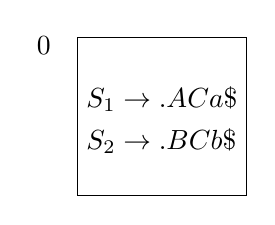
\begin{tikzpicture}
   \path (0,0) node[draw,shape=rectangle] (S0) 
   {
     \parbox{0\textwidth}{\begin{align*}
     & S_1 \rightarrow . A C a \$\\
     & S_2 \rightarrow . B C b \$
     \end{align*}}
   };
   \path (-1.5,0.9) node (S0n) {0};
\end{tikzpicture}
\caption{An example root state node in the parser generator.}
\end{figure}

The period shown on the right hand side of each rule is a cursor indicating the progress of the rule in a particular parser state.
For example, given an item $W_1 \rightarrow x . y$, this would indicate that the terminal $x$ has been recognized, and only $y$ remains to be parsed in order to recognize this rule.\\

\subsubsection{Expanding a state node}
Once an initial state node has been constructed the main loop of the construction algorithm is executed on the graph.
The root state is expanded until a nondeterministic \emph{branch state} is reached where the parser would be required to make a choice corresponding to the $switch$ operation.
During the expansion process parsing instructions are recorded into an \emph{instruction table} where each row consists of a string of instructions.
This array will be encoded into a bitcode stream once the algorithm completes.
Each \emph{instruction string} corresponds to a particular branch state in the state graph.
An alternative view of this idea is that every instruction string could represent a procedure of a recursive ascent parser written in an imperative programming language.\\

The following steps iteratively expand the state until a branch state is reached.

\begin{enumerate}
\item Expand items --- The token directly to the right of every cursor is inspected. 
If the token is a nonterminal token, then the item is replaced with the following items.
\begin{itemize} 
\item For every rule producing this nonterminal on the left, duplicate the item and annotate it with this rule number.
\item In addition a new item corresponding with the given rule and a cursor in the initial position should be added to the state whenever an old item is annotated. 
An exception is made only when such an item already exists in the state, in which case only the annotation takes place.
\end{itemize}
Once this process is completed the newly added (unannotated) items are again expanded until no more unnanoted items with nonterminals following a cursor can be found. 
For example, following the expansion procedure our example state will look like this.

\begin{figure}[!ht]
\centering
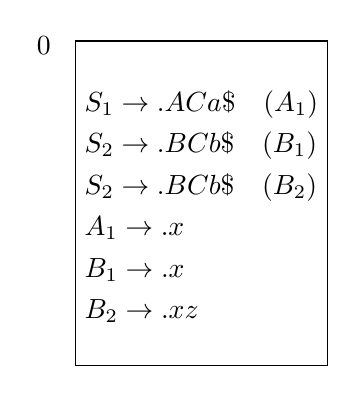
\begin{tikzpicture}
   \path (0,0) node[draw,shape=rectangle] (S) 
   {
     \parbox{0\textwidth}{\begin{align*}
     & S_1 \rightarrow . A C a \$ \quad {(A_1)}\\
     & S_2 \rightarrow . B C b \$ \quad {(B_1)}\\
     & S_2 \rightarrow . B C b \$ \quad {(B_2)}\\
     & A_1 \rightarrow . x\\
     & B_1 \rightarrow . x\\
     & B_2 \rightarrow . x z
     \end{align*}}
   };
   \path (-2,2) node (S0n) {0};
\end{tikzpicture}
\caption{Expanded items annotated with rule numbers.}
\end{figure}

Notice that there are two instances of the rule $S_2 \rightarrow . B C b \$$ annotated with the rules $(B_1)$ and $(B_2)$.

\item Shift terminal tokens --- Once all items have been expanded, each item is once again inspected. 
If a terminal token follows the cursor, it is moved one token forward and the terminal token is placed into a temporary set to be recognized.
For historical reasons, the set is known as the \emph{FIRST} set\footnote{$LR(k)$ parsers make a distinction between FIRST set and FOLLOW sets indicating, respectively, 
the first terminal tokens that can be recognized in a string of grammar tokens and the sets of terminals that could follow each of the FIRST terminals.} of the current state.
Because there must be at least one terminal token in the grammar (specifically the end-of-stream token \$) there is at least one token in the FIRST set.
If only one unique terminal exists in the set, then the state is \emph{deterministic} and hence a $shi\!ft$ instruction will be generated and appended to the corresponding string of instructions in the instruction table.
However, if multiple unique terminals exist in the FIRST set of the state, then the state is a non-deterministic branch state and a $switch$ instruction is generated instead.
\begin{itemize}
\item Given that a $shi\!ft$ instruction must be generated, the tool checks whether all items in the state are \emph{complete} in the sense described below. 
If they are not then the entire procedure is repeated until a set of FIRST terminals must once again be shifted. 
Otherwise, the tool returns to the state that preceded this one.
\item Given that a $switch$ instruction must be generated, the current state must be duplicated once for every unique terminal in the switch. 
A switch edge labeled with the terminal token connects every new state to its source.
However, every duplicate state must be filtered so that only the rules partaking in a particular branch of the switch are included.
All other items are removed from the new state. %TODO: more detail on this "filter"??
\end{itemize}

\item Complete items --- An item is \emph{completed} once the cursor has moved past all remaining tokens on the right hand side of the rule.
Once a $shi\!ft$ or a $switch$ has been generated, several items in the state may be completed. 
A separate subroutine called $CompleteItems$ is responsible for handling these completed items.
In the case of a $shi\!ft$ instruction, the items in the original state are completed whereas, in the case of a $switch$, each of the new states are processed by the routine.\\

When one or more items have been completed the generator must produce either a $reduce$ instruction indicating that a specific rule has been deduced or a $delay$ instruction when the rule to deduce is not yet clear.
The $delay$ instruction is produced whenever two or more rules are available for reduction or when one rule has a terminal token following its cursor indicating that the reduction might not take place at all.

The subroutine divides the set of items into two sets of completed items and incomplete items.
If none of the items in the state are completed then $CompleteItems$ exits returning false and the previous two steps are repeated.
Alternatively, if there is more than one unique item in the set of completed items or if there is only one unique item, but some incomplete items have terminals following their cursors then a $delay$ instruction is output.
\end{enumerate}

For example, iterative application of steps 1 to 3 will result in the following state changes.

\begin{figure}[!ht]
\centering
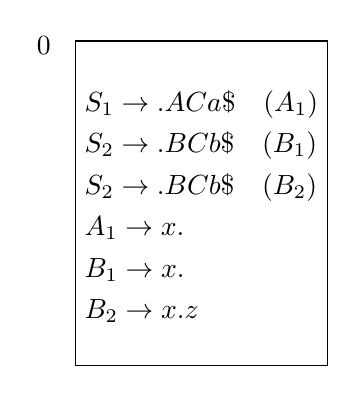
\begin{tikzpicture}
   \path (1,0) node[draw,shape=rectangle] (S) 
   {
     \parbox{0\textwidth}{\begin{align*}
     & S_1 \rightarrow . A C a \$ \quad {(A_1)}\\
     & S_2 \rightarrow . B C b \$ \quad {(B_1)}\\
     & S_2 \rightarrow . B C b \$ \quad {(B_2)}\\
     & A_1 \rightarrow x .\\
     & B_1 \rightarrow x .\\
     & B_2 \rightarrow x . z
     \end{align*}}
   };
   \path (-1,2) node (S0n) {0};
\end{tikzpicture}

\vspace{.5\baselineskip}
\small{\begin{tabular}{|c|l|}
  \hline
  \textbf{State} & \textbf{Instructions} \\
  \hline
  0 & $shift(x)$ \\ 
  \hline
\end{tabular}}
\caption{A $shi\!ft$ instruction is deduced by stepping over the $x$ terminal.}
\end{figure}

\begin{figure}[!ht]
\vspace{1\baselineskip}
\centering
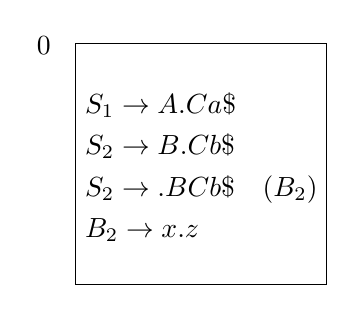
\begin{tikzpicture}
   \path (1,0) node[draw,shape=rectangle] (S) 
   {
     \parbox{0\textwidth}{\begin{align*}
     & S_1 \rightarrow A . C a \$ \quad \\
     & S_2 \rightarrow B . C b \$ \quad \\
     & S_2 \rightarrow . B C b \$ \quad {(B_2)}\\
     & B_2 \rightarrow x . z
     \end{align*}}
   };
   \path (-1,1.5) node (S0n) {0};
\end{tikzpicture}

\vspace{.5\baselineskip}
\small{\begin{tabular}{|c|l|}
  \hline
  \textbf{State} & \textbf{Instructions} \\
  \hline
  0 & $shift(x), delay(A_1, B_1)$ \\ 
  \hline
\end{tabular}}

\caption{A $delay$ instruction is deduced by completing rules $A_1$ and $B_1$. Take note of rule $B_2$ which cannot be completed due to the remaining terminal $z$.}
\end{figure}

\begin{figure}[!ht]
\vspace{1\baselineskip}
\centering
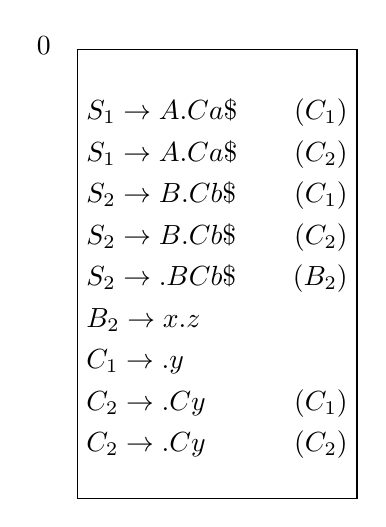
\begin{tikzpicture}
   \path (0,0) node[draw,shape=rectangle] (S)
   {
     \parbox{0\textwidth}{\begin{align*}
     & S_1 \rightarrow A . C a \$ & \quad {(C_1)}\\
     & S_1 \rightarrow A . C a \$ & \quad {(C_2)}\\
     & S_2 \rightarrow B . C b \$ & \quad {(C_1)}\\
     & S_2 \rightarrow B . C b \$ & \quad {(C_2)}\\
     & S_2 \rightarrow . B C b \$ & \quad {(B_2)}\\
     & B_2 \rightarrow x . z	    & \\
     & C_1 \rightarrow . y        & \\
     & C_2 \rightarrow . C y      & \quad {(C_1)}\\
     & C_2 \rightarrow . C y      & \quad {(C_2)}
     \end{align*}}
   };
   \path (-2.2,2.9) node (S0n) {0};
\end{tikzpicture}

\vspace{.5\baselineskip}
\small{\begin{tabular}{|c|l|}
  \hline
  \textbf{State} & \textbf{Instructions} \\
  \hline
  0 & $shift(x), delay(A_1, B_1)$ \\
  \hline
\end{tabular}}
\caption{Expand items with nonterminals following their cursors.}
\end{figure}

%\begin{figure}[!ht]
%\vspace{1\baselineskip}
%\centering
%\begin{tikzpicture}
%  \path (0,0) node[draw,shape=rectangle] (S)
%   {
%     \parbox{0\textwidth}{\begin{align*}
%     & S_1 \rightarrow A . C a \$ & \quad {(C_1)}\\
%     & S_1 \rightarrow A . C a \$ & \quad {(C_2)}\\
%     & S_2 \rightarrow B . C b \$ & \quad {(C_1)}\\
%     & S_2 \rightarrow B . C b \$ & \quad {(C_2)}\\
%     & S_2 \rightarrow . B C b \$ & \quad {(B_2)}\\
%     & B_2 \rightarrow x .z	    & \\
%     & C_1 \rightarrow y .        & \\
%     & C_2 \rightarrow . C y      & \quad {(C_1)}\\
%     & C_2 \rightarrow . C y      & \quad {(C_2)}
%     \end{align*}}
%   };
%   \path (-2.2,2.9) node (S0n) {0};
%\end{tikzpicture}
%
%\vspace{.5\baselineskip}
%\small{\begin{tabular}{|c|l|}
%  \hline
%  \textbf{State} & \textbf{Instructions} \\
%  \hline
%  0 & $shift(x), delay(A_1, B_1), switch(y \mapsto \textellipsis, z \mapsto \textellipsis)$ \\
%  \hline
%\end{tabular}}
%\caption{A $switch$ instruction is deduced by stepping over terminals $y$ and $z$.}
%\end{figure}

\clearpage
Now the example state has reached the `branch state' in which new states must be generated in order to continue. Hence two new states along with switch edges labeled $y$ and $z$ are generated as described in step 2 above.

\begin{figure}[!ht]
\centering
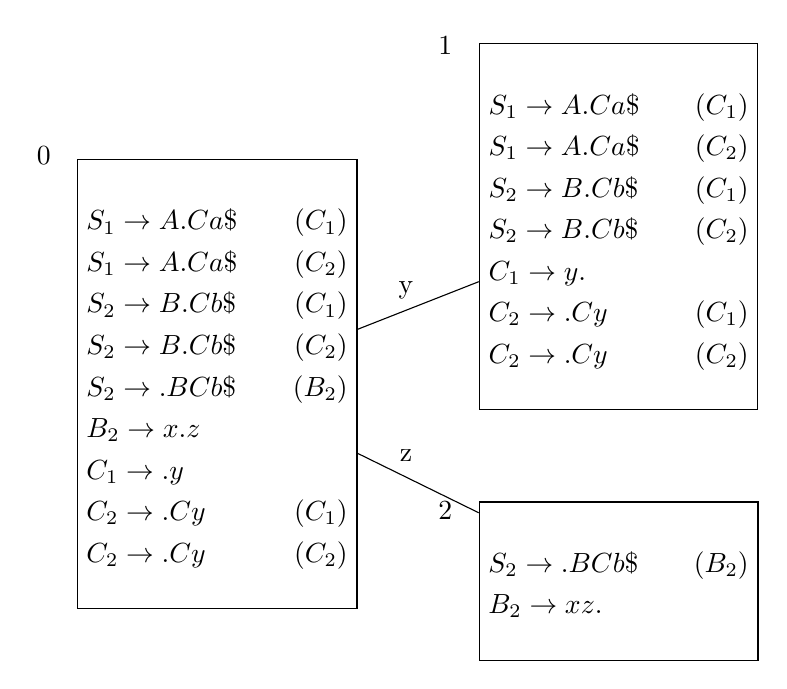
\begin{tikzpicture}
   \path (0,0) node[draw,shape=rectangle] (S0) 
   {
     \parbox{0\textwidth}{\begin{align*}
     & S_1 \rightarrow A . C a \$ & \quad {(C_1)}\\
     & S_1 \rightarrow A . C a \$ & \quad {(C_2)}\\
     & S_2 \rightarrow B . C b \$ & \quad {(C_1)}\\
     & S_2 \rightarrow B . C b \$ & \quad {(C_2)}\\
     & S_2 \rightarrow . B C b \$ & \quad {(B_2)}\\
     & B_2 \rightarrow x . z	    & \\
     & C_1 \rightarrow . y        & \\
     & C_2 \rightarrow . C y      & \quad {(C_1)}\\
     & C_2 \rightarrow . C y      & \quad {(C_2)}
     \end{align*}}
   };
   \path (-2.2,2.9) node (S0n) {0};

   \path (5.1,2.0) node[draw,shape=rectangle] (S1) 
   {
     \parbox{0\textwidth}{\begin{align*}
     & S_1 \rightarrow A . C a \$ & \quad {(C_1)}\\
     & S_1 \rightarrow A . C a \$ & \quad {(C_2)}\\
     & S_2 \rightarrow B . C b \$ & \quad {(C_1)}\\
     & S_2 \rightarrow B . C b \$ & \quad {(C_2)}\\
     & C_1 \rightarrow y .        & \\
     & C_2 \rightarrow . C y      & \quad {(C_1)}\\
     & C_2 \rightarrow . C y      & \quad {(C_2)}
     \end{align*}}
   };
   \path (2.9,4.3) node (S1n) {1};

   \path (5.1,-2.5) node[draw,shape=rectangle] (S2) 
   {
     \parbox{0\textwidth}{\begin{align*}
     & S_2 \rightarrow . B C b \$ & \quad {(B_2)}\\
     & B_2 \rightarrow x z .
     \end{align*}}
   };
   \path (2.9,-1.6) node (S2n) {2};

   %todo:  arrows...
   \path (2.4,1.2) node (ES0S1) {y};
   \path (2.4,-0.9) node (ES0S2) {z};
   \draw (S0) -- (S1) (S0) -- (S2);
\end{tikzpicture}

\vspace{.5\baselineskip}
\small{\begin{tabular}{|c|l|}
  \hline
  \textbf{State} & \textbf{Instructions} \\
  \hline
  0 & $shift(x), delay(A_1, B_1), switch(y \mapsto 1, z \mapsto 2)$ \\
  1 & $ $ \\ 
  2 & $ $ \\  
  \hline
\end{tabular}}
\caption{A $switch$ instruction is deduced by stepping over terminals $y$ and $z$ and two new states are generated.}
\end{figure}

\clearpage
Once the new states have been generated the process is repeated again on each of these. We demonstrate this up to the first $switch$ for states 1 and 2 below.

\begin{figure}[!ht]
\centering
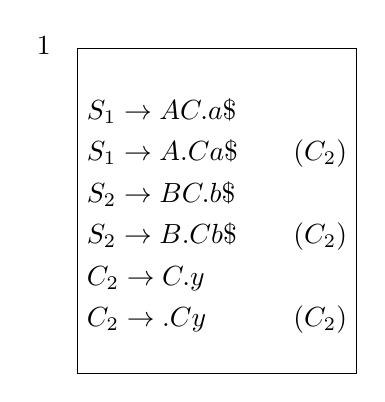
\begin{tikzpicture}
   \path (0,0) node[draw,shape=rectangle] (S1) 
   {
     \parbox{0\textwidth}{\begin{align*}
     & S_1 \rightarrow A C . a \$ & \quad \\
     & S_1 \rightarrow A . C a \$ & \quad {(C_2)}\\
     & S_2 \rightarrow B C . b \$ & \quad \\
     & S_2 \rightarrow B . C b \$ & \quad {(C_2)}\\
     & C_2 \rightarrow C . y      & \\
     & C_2 \rightarrow . C y      & \quad {(C_2)}
     \end{align*}}
   };
   \path (-2.2,2.1) node (S1n) {1};
\end{tikzpicture}

\vspace{.5\baselineskip}
\small{\begin{tabular}{|c|l|}
  \hline
  \textbf{State} & \textbf{Instructions} \\
  \hline
  0 & $shift(x), delay(A_1, B_1), switch(y \mapsto 1, z \mapsto 2)$ \\
  1 & $reduce(C_1), switch(a \mapsto \textellipsis, b \mapsto \textellipsis, y \mapsto \textellipsis)$ \\ 
  2 & $ $ \\  
  \hline
\end{tabular}}
\caption{State 1 after iteratively applying steps 1 to 3.}
\end{figure}

\begin{figure}[!ht]
\vspace{1\baselineskip}
\centering
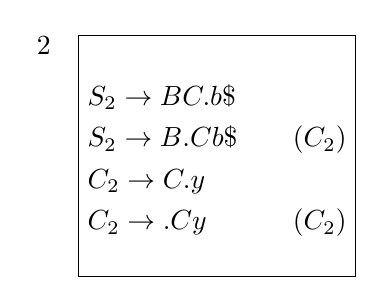
\begin{tikzpicture}
   \path (0,0) node[draw,shape=rectangle] (S2) 
   {
     \parbox{0\textwidth}{\begin{align*}
     & S_2 \rightarrow B C . b \$ & \\
     & S_2 \rightarrow B . C b \$ & \quad {(C_2)}\\
     & C_2 \rightarrow C . y      & \\
     & C_2 \rightarrow . C y      & \quad {(C_2)}
     \end{align*}}
   };
   \path (-2.2,1.4) node (S2n) {2};
\end{tikzpicture}

\vspace{.5\baselineskip}
\small{\begin{tabular}{|c|l|}
  \hline
  \textbf{State} & \textbf{Instructions} \\
  \hline
  0 & $shift(x), delay(A_1, B_1), switch(y \mapsto 1, z \mapsto 2)$ \\
  1 & $reduce(C_1), switch(a \mapsto \textellipsis, b \mapsto \textellipsis, y \mapsto \textellipsis)$ \\ 
  2 & $reduce(B_2), shift(y), reduce(C_1), switch(b \mapsto \textellipsis, y \mapsto \textellipsis)$ \\  
  \hline
\end{tabular}}
\caption{State 2 after iteratively applying steps 1 to 3.}
\end{figure}

\clearpage
The following pseudo-code describes the details of this procedure in a more concrete manner.

%\begin{figure}
\begin{center}
\begin{gcl}
\PROC ConstructStateGraph(stateGraph, grammarRules, startNonterminal)
  stateGraph_0 \becomes GetStartItems(grammarRules, startNonterminal)
  ExpandStateGraph(stateGraph, grammarRules)
\CORP

\PROC ExpandStateGraph(stateGraph, grammarRules)
  allItemsComplete \becomes false;
  \DO allItemsComplete \neq true \rightarrow
    ExpandItems(stateGraph_0, grammarRules, 0, stateGraph_{0}.items.length);
    ShiftTerminals(stateGraph_0);
    allItemsComplete \becomes CompleteItems(stateGraph, state);
  \OD

   \{ \text{Expand the newly generated states}\textellipsis \}
  ExpandStateGraph(\textellipsis)
\CORP

\PROC ExpandItems(state, grammarRules, begin, end)
  \{ \text{Add rule annotations and create new items.} \}
  i \becomes begin;
  \DO i < end \rightarrow
    \IF state.items_{i}.ruleAnnotation = nil 
    \land \neg IsTerminal(rhsToken)
    \land \neg IsComplete(state.items_i) \rightarrow
    \quad rhsToken \becomes items_{i}.rule.RHS_{state.items_{i}.cursor};
    \quad j \becomes 0;
    \quad \DO j < productions_{rhsToken}.rules.size \rightarrow
          % if an un-annotated item, annotate it. Otherwise add another annotated item
          \IF state.items_{i}.ruleAnnotation = nil \rightarrow
          \quad \{ \text{Replace the existing item's annotation.} \}
          \quad state.items_{i}.ruleAnnotation \becomes productions_{rhsToken}.rules_j;
          \BAR state.items_{i}.ruleAnnotation \neq nil \rightarrow
          \quad \{ \text{Duplicate the item and set the annotation.} \}
          %\quad state.items_{state.items.size} \becomes state.items_{i};
          \quad state.items.Append(state.items_{i});
          \quad state.items_{state.items.size}.ruleAnnotation \becomes productions_{rhsToken}.rules_j;
          \FI
          \{ \text{Create a new item if it does not exist yet.} \}
          newItem \becomes Item(productions_{rhsToken}.rules_j);
          \IF newItem \in state.items \rightarrow \SKIP;
          \BAR newItem \notin state.items \rightarrow state.items.Append(newItem);
          \FI
          j \becomes j + 1;
        \OD
    \BAR state.items_{i}.ruleAnnotation \neq nil
    \lor IsTerminal(state.items_{i}.rule.RHS_{state.items_{i}.cursor})
    \lor IsComplete(state.items_{i}) \rightarrow  
      \quad \SKIP;
    \FI
    i \becomes i + 1;
  \OD

  \{ \text{Expand all newly created items.} \}
  \IF state.items.length > end \rightarrow 
    ExpandItems(stateGraph_0, grammarRules, end, state.items);
  \BAR state.items.length = end \rightarrow 
    \SKIP;
  \FI
\CORP

\PROC ShiftTerminals(state)
  \{ \text{Determine whether to generate a shift instruction or a switch instruction.} \}
  firstSet \becomes ProcessFirstTerminals(state);
  \IF firstSet.size = 1 \rightarrow GenerateShiftInstruction(state, firstSet);
  \BAR firstSet.size > 1 \rightarrow GenerateSwitchInstruction(state, firstSet);
  \FI
\CORP

\PROC CompleteItems(state, grammarRules)
  \{ \text{Split the state into two sets of complete and incomplete items.} \}
  waitingShiftActions \becomes false;
  completeItems \becomes \{\};
  incompleteItems \becomes \{\};
  i \becomes 0;
  \DO i < state.items.length \rightarrow
    \IF IsComplete(state.items_i) \rightarrow
      completeItems.Insert(state.items_i);
    \BAR \neg IsComplete(state.items_i) \rightarrow
      incompleteItems.Insert(state.items_i);
      \IF IsTerminal(state.items_i.RHS_{state.items_{i}.cursor}) \rightarrow
          waitingShiftActions \becomes true;
        \BAR \neg IsTerminal(state.items_i.RHS_{state.items_{i}.cursor}) \rightarrow
          \SKIP;
      \FI
    \FI
    i \becomes i + 1;
  \OD

  \{ \text{Generate reduce / delay instructions.} \}
  \IF completeItems.size = 0 \rightarrow 
    \SKIP;
  \BAR completeItems.size = 1 \land waitingShiftActions = false \rightarrow 
    GenerateReduceInstruction(state, completeItems);
  \BAR completeItems.size > 0 \lor waitingShiftActions = true \rightarrow 
    GenerateDelayInstruction(state, completeItems);
    state.delayedStack.Push(completeItems);
  \FI

  \{ \text{Remove completed items from the state.} \}
  i \becomes 0;
  \DO i < state.items.length \rightarrow
    \IF IsComplete(state.items_i) \rightarrow
      state.items.Remove(state.items_i);
    \BAR \neg IsComplete(state.items_i) \rightarrow
      i \becomes i + 1;
    \FI
  \OD

  \{ \text{Step over completed nonterminals and duplicate incomplete items.} \}
  i \becomes 0;
  \DO i < state.items.length \rightarrow
    \IF state.items_i.ruleAnnotation \in completeItems.rules \rightarrow
      newItem \becomes state.items_i;
      state.items_i.cursor \becomes state.items_i.cursor + 1;
      state.items_i.ruleAnnotation \becomes nil;
      \IF state.items_i.ruleAnnotation \in incompleteItems.rules \rightarrow
        state.items.Append(newItem);
      \BAR state.items_i.ruleAnnotation \notin incompleteItems.rules \rightarrow
        \SKIP;
      \FI
    \BAR state.items_i.RHS_{state.items_i.cursor} \notin completeItems.rules \rightarrow
      \SKIP;
    \FI
    i \becomes i + 1;
  \OD

  \{ \text{Complete all remaining incomplete items.} \}
  \IF completeItems.size > 0 \rightarrow
    \textbf{return} \ CompleteItems(state, grammarRules);
  \BAR completeItems.size = 0 \rightarrow
    \textbf{return} \ false;
  \FI
\CORP

\end{gcl}
%\caption{State graph expansion.}
\end{center}
%\end{figure}

\subsubsection{Handling cycles}
Most useful grammars contain cycles where a pattern may be repeated. Attempting to expand the state graph for a cycle would repeat infinitely.
To overcome this a modification must be made where the generator checks for a previous node with an identical branch state. 
If a cycle can be established then the algorithm generates switch edges to the same targets that the previous node has. 
Additional $return$ instructions must also be appended to each state in order for recursion to take place.

\subsubsection{Generating $goto$ and $resolve$ instructions}
In order to implement the lookahead mechanism, $goto$ instructions must also be generated by the algorithm.
After the state graph has been fully expanded, additional goto edges and state nodes are added by a separate step.
Each state will also contain a stack of delayed rules recorded in the previous steps.
The algorithm must traverse the graph generating $resolve$ instructions where possible. 
If a rule is resolved in a different cycle depth then new states are generated with $goto$ edges connecting them to their origins.

%In the final section of this paper we will discuss the limitations of this algorithm and discuss some proposals for extension that take into account the full set of context free grammars. 
%(TODO: We will also show that parsers built using this technique already includes the entire class of $LR(1)$ grammars)

\section{Results}

It is tempting to classify an LD parser performance according to the number of operations per input token.
However, the class of the grammar that the parser represents should also be taken into account for comparison with other parsers.
For simplicity only the recognition pass is considered here. 
The translation pass builds a parse tree in much the same way as any $LR(0)$ parser, therefore the expected worstcase performance is $O(n)$.

Analyzing the performance of each instruction individually is relatively straightforward. 
For this reason it is easiest to characterize the performance of LD parsers according to the number of parsing instructions an LD parser may take.
The table below lists the performance of each individual operation according to its arguments.
\clearpage
\begin{table}[!ht]\centering
  \begin{tabular}{|l|l|}
  \hline
  \textbf{Operation} & \textbf{Time} \\
  \hline
  $shi\!ft$          & constant \\ \hline
  $switch$           & linear in the number of arguments \\ \hline
  $accept$/$return$  & constant \\ \hline
  $goto$             & linear in the number of arguments \\ \hline
  $delay$            & constant \\ \hline
  $reduce$           & constant \\ \hline
  $resolve$          & constant \\
  \hline
  \end{tabular}
\caption{Performance of individual parsing operations.}
\end{table}

It is possible for the operations that exhibit linear time performance, $shi\!ft$ and $goto$, to encode their arguments in a flattened binary tree or perform similar tricks in order to decrease asymptotic access time.
However, the overhead of the additional operations and memory access is likely to dominate performance in practice since the number of arguments are expected to be few.
It is common practice to reduce these very basic recognition operations to constant time operations since the number of arguments given to an instruction is fixed with respect to the number of input tokens.

Given an input stream of $n$ tokens, every token in the input stream may only be tested once during the recognition pass.
Hence, the number of $shi\!ft$ and $switch$ operations executed by the parse will certainly be linear in $n$.

The number of reductions that take place seem intuitively related to both the number input tokens and the complexity of the given grammar specification.
However, since $reduce$ instructions do not take any lookahead into account $reduce$ instructions should have the same worst-case asymptotic performance regardless of the class of grammar used.
The performance can be related to $n$, the number of input tokens, and $j$, the maximum depth of the final parse tree.

Consider cases in which the grammar falls within the class $LR(k)$ for some fixed $k$.
In the worst case the number of $reduce$ operations will be $(j - 1) \cdot n + 1$ since every token will be involved in at most $j$ productions, one of which has to be the root node of the parse tree.
When the grammar is unambiguous the number of rules with only nonterminals on the right hand side will necessarily be constant.
Since every rule that is not one of these must consume at least one terminal, most analyses simply reduce $j$ to a constant term.
Therefore, for all unambiguous grammars the number of $reduce$ operations is roughly linear with respect to the number of input tokens.

%From a practical point of view we expect that sane grammars will not include many redundant \emph{alternative wording?} productions, especially inside recursive rules.
%Based on this assumption, it is our estimation that a typical average case performance of $o(n)$ is far more likely for most applications. (An argument that could most likely be applied to GLR and Earley parsers as well).

The pair of actions $delay$ and $resolve$ should exhibit similar performance to $reduce$.
We have already seen that the equivalent trace using delays may split a $reduce$ operation into a single pair of $delay$ and $resolve$ operations.
The only difference here is that some delay actions may be resolved using an $ignore$ which does not correspond to any $reduce$ operation.
An $ignore$ token may be generated through a $resolve$ whenever two or more rules are evaluated simultaneously with lookahead. 
Using the same argumentation showing that $reduce$ is $O(n)$ with respect to the number of input tokens it can be seen that the number of possible reductions in any one of these rules is linear.
Assuming that the number of these simultaneous rules will be constant\footnote{An assertion that may require further investigation.}, the number of $ignore$ tokens will also be linear.

Finally, determining the upper limit for $return$ and $goto$ operations is trivial once one realizes that both operations must correspond to a preceding $switch$ operation. 
It follows that $return$ and $goto$ are both linear in $n$.\\

All of the above arguments seem to indicate that LD parsers can be constructed that will perform in linear---or at least near-linear---time for those unambiguous grammars that can be parsed using the instruction set.
Our initial performance analysis appears favourable in comparison to the most efficient generalized parsing algorithms.

\section{Conclusions}

In the course of this work we have designed and implemented a new framework for building parsers using a novel lookahead mechanism.
Following some refinement our methodology has been distilled into a simple, easily understood set of instructions.
Modeling the parser as a domain specific language afforded us the opportunity to apply well known existing semantic models to parsers.
Although a little unexpected at first, we have come to the conclusion that concepts from programming language theory may be ideal for studying parsing.
This is not so suprising in retrospect given that grammars have a lot in common with programs and suffer from similar decidability issues.

The distinction made between language recognition and language translation allowed us to separate these two concerns into separate passes, 
thereby simplifying lookahead greatly. %\emph{TODO: Another contribution is the recognition of the longest non-deterministic strings ...}

From an implementation point of view, a parser driver was implemented consisting of a lexer, parser interpreter and a tree builder.
In addition to this a prototype parser generator tool was implemented using our current work-in-progress construction algorithm.
Parsing instructions are encoded into a small bitcode format by the parser generator and passed to the interpreter by the parser driver.
Every parsing operation in the interpreter is small and simple and all auxiliary data structures are similarly uncomplicated. 
Therefore it is our hope and expectation that the interpreter will perform well in comparison to other automatically generated parsers, especially where generalized parsing is concerned.

\section{Future work}

We consider our work thus far to be exploratory in nature.
As such, there remains a large amount of theoretical and practical work to be done.
Our main concern is increasing the generality of LD parsing in order to handle a larger class of context-free grammars, possibly including all ambiguous grammars. 
It should be noted that it is possible to annotate $delay$ operations with the possible reductions that could be performed at this step.
We see a possibility for future work in generating new rule numbers for various combinations of delayed rules, using these in place of the usual $ignore$ placeholder token.

%Another interesting problem related to parsing that we feel may be related to our work is the translation from one grammar to another.
%If such a translator could be automatically generated by encoding it in some kind of grammar then a powerful lookahead mechanism such as the one presented here could be used.
%While this idea is pure conjecture, perhaps such a translator could be used to automatically generate complex transformations inside optimizing compilers.

It has been demonstrated that the LD instruction set is capable of handling a wide variety of unambiguous context-free grammars but will not accept the special case where lookahead is required outside multiple nested cycles.
We put forward the idea that the instruction set might be extended, possibly by adding an alternative to the $return$ instruction that does not remove the last address from the callstack.

Knuth showed that determining whether a context-free grammar is ambiguous is undecidable in general\cite{knuth65}. 
This implies that certain concequences must be taken into account in our work. 
First off, determining whether a grammar is a suitable candidate for parsing using our current instruction set seems to be undecidable.
Although we have not yet experienced this problem we suspect that the issue may manifest as infinite growth in the state graph during the construction algorithm if certain grammars are used.
If this effect does occur it can simply be circumvented by specifying a limiting depth for the generator to use. 
Even so, this possibility warrants further study.

In the Results section a rough analysis of the performance of the LD parser was given.
The simplicity of our approach emboldens us to profile the efficiency of generated parsers.
Benchmarks should be set up in order to test the performance of generated parsers in comparison to other parser generators.
While asymptotic performance gives a useful metric of the scalability of parsing algorithms in various scenarios, the constant term tends to have a large effect on parsing performance in practice.
Furthermore, complex effects such as memory latency and branch misprediction will be missed by over-simplified mathematical models.
Many opportunities for optimization are still available, especially where construction of the parsers are concerned.
Another possibility that could provide additional speedup is direct conversion of parsers to machine code using an optimizing compiler.
%Much of the research into parsing algorithms occured in the 70's. 
%Today's hardware has different performance characteristics which is still in a phase of rapid change. 
%In order to take advantage of modern hardware, now and in the future, we may need to re-evaluate the classical algorithms using different performance metrics.
%In order to take advantage of modern hardware, now and in the future, we may need to re-evaluate the classical algorithms using different performance metrics.

Finally, there are additional engineering concerns that also need to be resolved before LD parsing can be considered for industrial use.
In particular we have omitted error recovery, semantic actions, precedence rules and incremental parsing from our work thus far.

%\emph{ %BUSY HERE
%(TODO)\\
%Open problems: problematic unambiguous context-free grammars (nested lookahead problem + construction problem), progressive parsing (combining the recognition and builder passes), formal proofs of correctness\\
%Suggest that delays should be encoded as stacks of continuations similar to functional programming rather than as a simple callstack?\\
%Performance analysis and benchmarks\\
%Termination analysis\\
%Proof is needed for the absence of exponential growth of states in the generated parser\\
%Parallelization / pipelined implementations?\\
%Application to other grammar classes (E.g. ambiguous context-free and context-sensitive grammars)\\
%}

\section*{Acknowledgements}
I would like to thank Prof. Derrick Kourie and Prof. Bruce Watson of the University of Pretoria for their insightful suggestions and patient support during the development of this work.

\bibliographystyle{plain}
\bibliography{delayedcase}

\end{document}

